\RequirePackage{amsthm}

\documentclass[sn-mathphys-num]{sn-jnl}

% Standard Packages
\usepackage{graphicx}%
\usepackage{natbib}
\usepackage{multirow}%
\usepackage{amsmath,amssymb,amsfonts}%
\usepackage{amsthm}%
\usepackage{mathrsfs}%
\usepackage[title]{appendix}%
\usepackage{xcolor}%
\usepackage{textcomp}%
\usepackage{manyfoot}%
\usepackage{booktabs}%
\usepackage{algorithm}%
\usepackage{algorithmicx}%
\usepackage{algpseudocode}%
\usepackage{listings}%
\usepackage{subcaption}

\theoremstyle{thmstyleone}%
\newtheorem{theorem}{Theorem}%  meant for continuous numbers
\newtheorem{proposition}[theorem]{Proposition}% 
\theoremstyle{thmstyletwo}%
\newtheorem{example}{Example}%
\newtheorem{remark}{Remark}%
\theoremstyle{thmstylethree}%
\newtheorem{definition}{Definition}%
\raggedbottom

\begin{document}
\title[Article Title]{Some Network for Medical Image Segmentation}

\author*[1,2]{\fnm{First} \sur{Author}}\email{iauthor@gmail.com}
\author[2,3]{\fnm{Second} \sur{Author}}\email{iiauthor@gmail.com}
\equalcont{These authors contributed equally to this work.}
\author[1,2]{\fnm{Third} \sur{Author}}\email{iiiauthor@gmail.com}
\equalcont{These authors contributed equally to this work.}
\affil*[1]{\orgdiv{Department}, \orgname{Organization}, \orgaddress{\street{Street}, \city{City}, \postcode{100190}, \state{State}, \country{Country}}}
\affil[2]{\orgdiv{Department}, \orgname{Organization}, \orgaddress{\street{Street}, \city{City}, \postcode{10587}, \state{State}, \country{Country}}}
\affil[3]{\orgdiv{Department}, \orgname{Organization}, \orgaddress{\street{Street}, \city{City}, \postcode{610101}, \state{State}, \country{Country}}}

\abstract{
Large amount of high-quality annotated data for training is required by medical image segmentation area, this limitation restricts their broader clinical use in disease diagnosis, treatment planning, and monitoring.
Semi-supervised learning (SSL) has recently emerged as a promising approach to address this challenge, enabling the utilization of both labeled and unlabeled data to improve segmentation performance.
Also, Segment Anything (SAM) from Meta has shown great potential in medical image segmentation, leveraging large-scale pretraining on diverse datasets to enhance model generalization.
However, existing SSL methods often rely on complex architectures and extensive computational resources, making them less practical for real-world applications.
}

\keywords{Medical Image Segmentation, Semi-Supervised Learning, Deep Learning}

\maketitle

\section{Introduction}\label{sec1}
% 介绍医学图像分割任务的重要性,以及全监督方法的弊端
Medical image segmentation plays a pivotal role in medical imaging by enabling precise delineation of anatomical structures and pathological regions.  
Accurate segmentation is indispensable for clinical applications, including disease diagnosis, treatment planning, and longitudinal monitoring of disease progression.  
Deep learning-based methods have revolutionized medical image segmentation, achieving remarkable success in various tasks.
However, these fully-supervised methods often face two main challenges:
(1) A large amounts of annotated data is required in training part, which is a significant limitation in clinical practice due to the time-consuming and labor-intensive nature of manual annotation.
(2) The performance of these methods heavily relies on the availability of high-quality annotated data, which is often scarce in many medical imaging tasks.
Besides, many commonly used medical images like computed tomography (CT) and magnetic resonance imaging (MRI) scans are 3D volumetric data, further increase the burden of manual annotation compared with 2D images.
Therefore, training deep learning models with limited annotated data remains a significant challenge in the field of medical image segmentation.

% 半监督学习过程
To address the challenge of limited annotated data, researchers have made substantial efforts in developing annotation-efficient methods in medical image segmentation.
Semi-supervised learning (SSL) could effectively leverage the information contained in both labeled and unlabeled data and improves model performance.
this method have shown great potential in medical image segmentation, enabling the utilization of both labeled and unlabeled data to improve segmentation performance.
there are mainly two types of SSL methods: consistency regularization and pseudo-labeling.
Using pseudo-labeling path,it could enlarge the training data through label generalization to improve stability of the model while training.
it also could use data augmentation and consistency regularization to enhance the model's robustness and generalization ability.
these methods have shown promising results in various medical image segmentation tasks, demonstrating their effectiveness in improving model performance with limited annotated data.

% Segment anything相关内容
Recent years have witnessed the emergence of foundation models in computer vision, notably represented by the Segment Anything Model (SAM) for 2D image segmentation, which demonstrates impressive zero-shot generalization capabilities across various natural image segmentation tasks.
However, because of the suubstantial domaingap, its performance remains suboptimal in medical images segmentation tasks.

% 介绍半监督和SAM当前面对的一些困难

% 提出自己的方法

\section{Relative works}\label{sec2}

\subsection{U-shaped CNNs Methods}
% 介绍U型卷积网络的相关方法
U-shaped convolutional neural networks are essential technology driving groundbreaking progress in the field of medical image segmentation, particularly for their powerful feature extraction capabilities. 
Jonathan Long et al. \cite{long2015fully} revolutionized segmentation with FCNs by replacing fully connected layers in traditional CNNs with convolutional layers, enabling segmentation for images of arbitrary sizes and significantly improving accuracy.
Olaf Ronneberger et al. \cite{ronneberger2015u} further extended this architecture with U-Net, adopting an encoder-decoder structure with skip connections.
The encoder gradually extracts features and downsamples the input, while the decoder upsamples the feature maps to recover resolution.
Skip connections allow low-level features to directly feed into the corresponding decoder stage, greatly enhancing the integration of multi-scale features \cite{aitken2021understanding}.
Milletari et al. \cite{milletari2016v} proposed that V-Net can better capture information on 3D space by using 3D convolution operations.
Zongwei Zhou et al. \cite{zhou2018unet++} introduced UNet++, a nested U-shaped architecture that optimizes feature transmission and integration through dense skip connections and multi-scale feature fusion.
Ange Lou et al. \cite{lou2021dc} proposed DC-UNet, this method incorporates a dual-channel design into the U-Net architecture to effectively combine multi-modal feature representations, resulting in substantial improvements in both segmentation performance for multi-modal medical images and computational efficiency.
Huimin Huang et al. \cite{huang2020unet} introduced UNet3+, the architecture leverages CNNs to dynamically combine low-level and high-level information, achieving efficient 3D medical image segmentation.
The U-shaped architecture has achieved remarkable results in medical image segmentation, we also adopted it to develop a multi-organ segmentation network.

\subsection{Attention-Based Methods}
% 介绍基于注意力的相关方法
Attention mechanisms were first applied in Natural Language Processing (NLP) and later introduced to computer vision, yielding promising results in tasks such as classification and detection.
This strategy dynamically adjusts the focus of the network on the feature map, significantly enhancing performance in complex visual tasks\cite{chen2019multi}.
Hu et al. \cite{hu2018squeeze} proposed the Channel Attention Mechanism (CAM), it dynamically adjusts the feature map along the channel dimension and improves the model's ability to evaluate feature importance.
Oktay et al. \cite{oktay2018attention} introduced the attention gate mechanism in U-Net, which dynamically weighs feature maps during the decoder stage, suppressing irrelevant background information and improving segmentation accuracy and robustness.
Dosovitskiy et al. \cite{dosovitskiy2020image} introduced the Vision Transformer (ViT) architecture, this work applies Transformer mechanisms to visual tasks by dividing images into patches, further advancing the field.
Chen et al. \cite{chen2021transunet} proposed combining the Transformer and U-Net structures, enhancing global feature modeling in the encoder while retaining multi-scale feature advantages.
Liu et al. \cite{liu2021swin} presented the Swin Transformer, which achieves efficient global feature modeling through a shifted window mechanism. 
Following this, Cao et al. \cite{cao2022swin} introduced the Swin-Unet architecture, integrating Swin Transformer modules into U-Net encoder and decoder stages, effectively utilizing local and global feature integration to improve segmentation accuracy and computational efficiency.
Also, Huang et al. \cite{huang2022missformer} proposed an enhanced transformer context bridge with the enhanced transformer block that extracts the long-range dependencies and local context of multi-scale features generated by a hierarchical transformer encoder.
This progress underlines the importance of global feature extraction to effectively tackle complex visual tasks in medical image segmentation.

\subsection{Lightweight-Based Methods}
% 介绍轻量化的相关工作
Despite significant advances in U-shaped CNNs and attention-based methods, there were still challenges with computational resources and efficiency.
It mainly dues to the complexity of CNNs and the non-linear increase in the computational cost of attention mechanisms in Transformer architectures as input image size increases \cite{zheng2024lightweight}.
To address these issues, Xie et al. \cite{xie2017aggregated} proposed ResNeXt, this architecture reduces the computational cost of convolutions by introducing grouped convolutions in image classification.
Grouped convolution significantly lowers computational complexity while maintaining model performance by dividing input features into groups.
Similarly, Howard et al. \cite{howard2017mobilenets} proposed MobileNet, which used depthwise and pointwise convolutions to reduce both parameter count and computational cost.
This technique has been widely adopted in mobile and embedded devices and serves as a foundation for lightweight convolutional network design. 
Ding et al. \cite{ding2021repvgg} demonstrated the effectiveness of large-kernel convolutions, this large-kernel can replace parts of the self-attention mechanism and preserve efficient convolution operations.
It also reduces computational complexity and retains the ability to model long-range dependencies.
Trockman et al. \cite{trockman2022patches} proposed ConvMixer, which uses large convolution kernels to mix distant spatial position information.
Wang et al. \cite{wang2021pyramid} introduced the PVT model, this model combines multi-scale local convolutions with global attention mechanisms.
Liu et al. proposed ConvNeXt \cite{liu2022convnet}, this work used large convolution kernels and Swin Transformer \cite{liu2021swin} architecture design tricks to improve the performance of fully convolutional networks in all aspects.
Tolstikhin et al. \cite{tolstikhin2021mlp} proposed UNeXt, which designed a lightweight medical image segmentation network based on a hybrid architecture of CNNs and multilayer perceptron.
Tang et al. \cite{tang2023cmu} demonstrated that ConvUNeXt leverages and improves the ConvNeXt block for efficient segmentation.
Guo et al. \cite{guo2023visual} proposed the Visual Attention Network, which incorporates large-kernel convolution attention, expanding the receptive field to capture broader contextual information.
However, while these lightweight methods have shown promising results in natural image processing, they still face challenges in medical image processing due to the differences in feature distribution between medical and natural images.	

\section{Method}\label{sec3}

\subsection{Architecture Overview}\label{subsec1}
% 简单介绍一下网络整体
As illustrated in Figure \ref{fig1}, the proposed network is primarily divided into an encoder and a decoder, this architecture adopts a multi-level U-shaped structure.

\begin{figure}[ht]
    \centering
    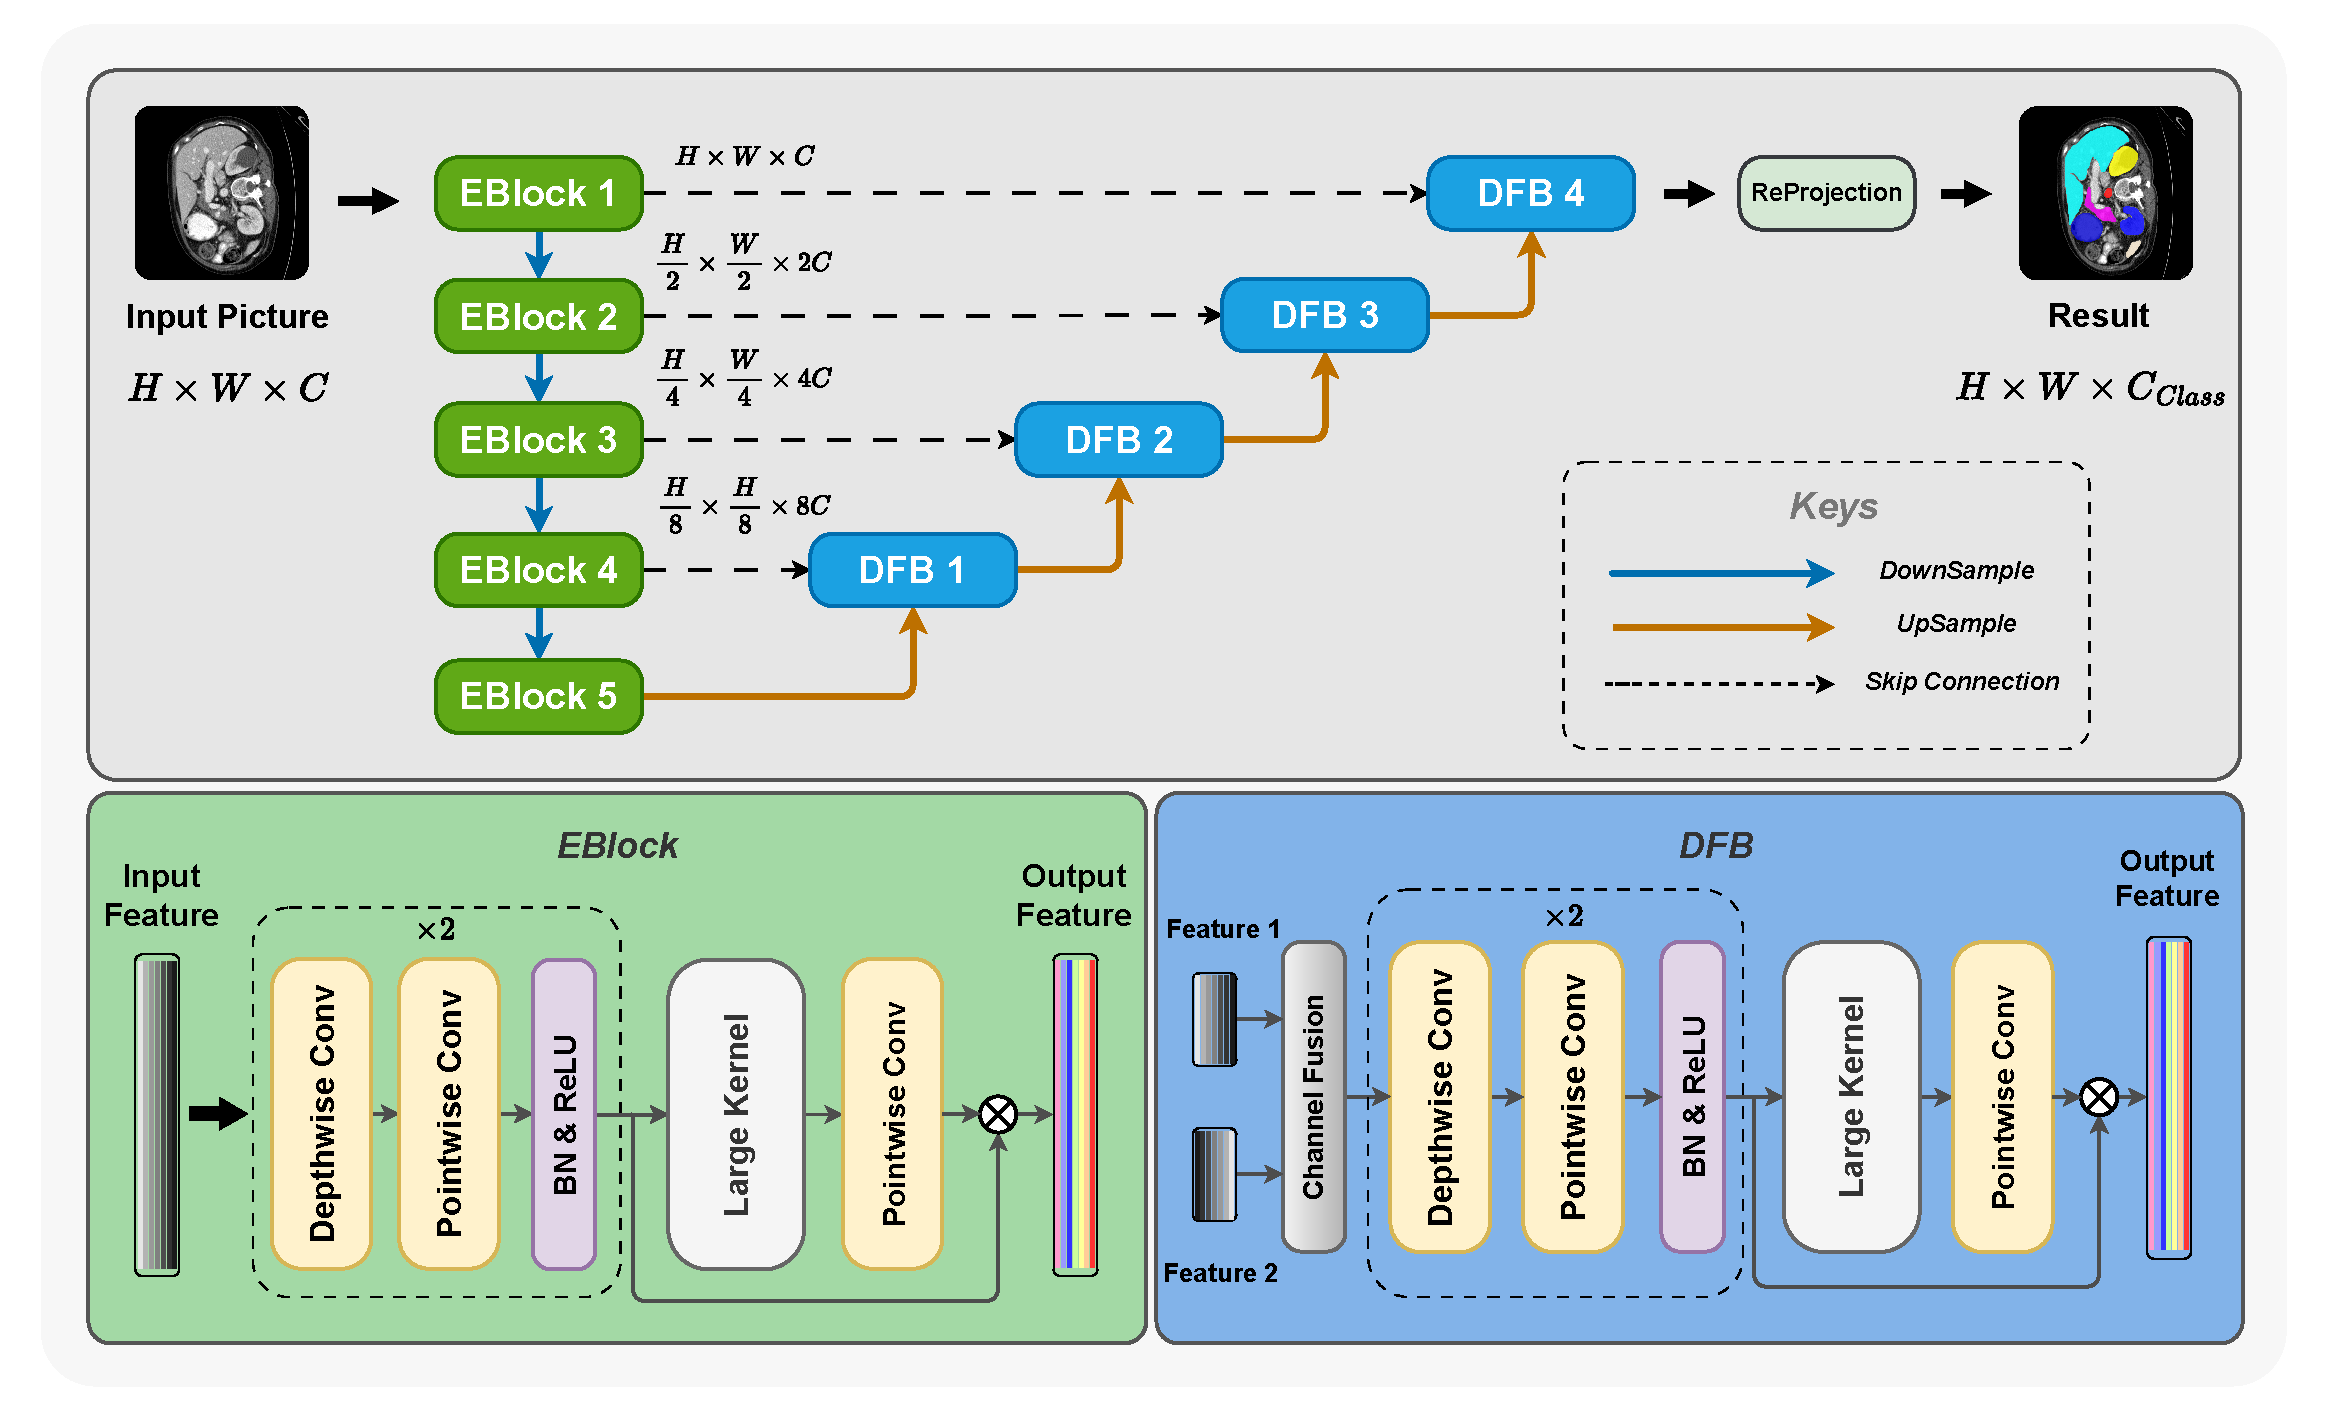
\includegraphics[width=\textwidth]{figure1.pdf}
    \caption{An illustration of \textbf{DLKUNet}, which is composed of encoder (\textcolor{green}{Green}), decoder (\textcolor{blue}{Blue}) and reprojection layer.
    The blue arrow represents the downsample between different modules in the encoder, and the orange arrow represents the upsample in the decoder.
    The two pictures below show the internal structure of \textbf{EBlock} and \textbf{DFB} respectively.}\label{fig1}
\end{figure}

% 介绍一下encoder与下采样过程
In the encoder, a progressive design strategy is employed to capture multi-scale information and effectively compress the feature representation of the input image.
The encoder consists of five DLKBlock layers and the first layer performs initial feature extraction by expanding the input feature channels to \(C\).
DLKBlock consists of downsampling operations and an Encoder Block(EBlock) in each encoder layer.
Similar to models like U-Net \cite{ronneberger2015u} and MobileVit \cite{howard2017mobilenets}, we decouple the downsampling layers to enhance training stability and overall model performance.
To keep better trade-off computational efficiency and accuracy, we use the max-pooling downsampling method with \(2\times 2\) kernel size and stride as \(2\).
This downsampling strategy retains crucial feature information while reducing computational complexity, thereby enhancing the effectiveness of the model in medical image segmentation.

% 介绍一下decoder与上采样过程
In the decoder, a stepwise design is adopted to maintain synergy with the encoder and restore feature details while ensuring model performance.
The decoder consists of four DLKBlock layers and a reprojection layer.
The reprojection layer is responsible for restoring the number of channels and refining the feature information, ultimately producing precise multi-class segmentation results.
Each DLKBlock in the decoder layer consists of a Decoder Fusion Block(DFB) and upsampling operations, primarily used to merge feature tensors from multiple pathways.
The upsampling process uses a transposed convolution with \(3\times 3\) kernel size, stride as 1, and padding as 1 to double the resolution of the feature maps.
This provides richer and more precise input data for subsequent processing.

\subsection{EBlock}\label{subsec2}
% 介绍一下EBlock的主要组成部分
As shown in Figure \ref{fig2}, The structure of the EBlock consists of two main components: the convolution part and the attention part. 

\begin{figure}[ht]
    \centering
    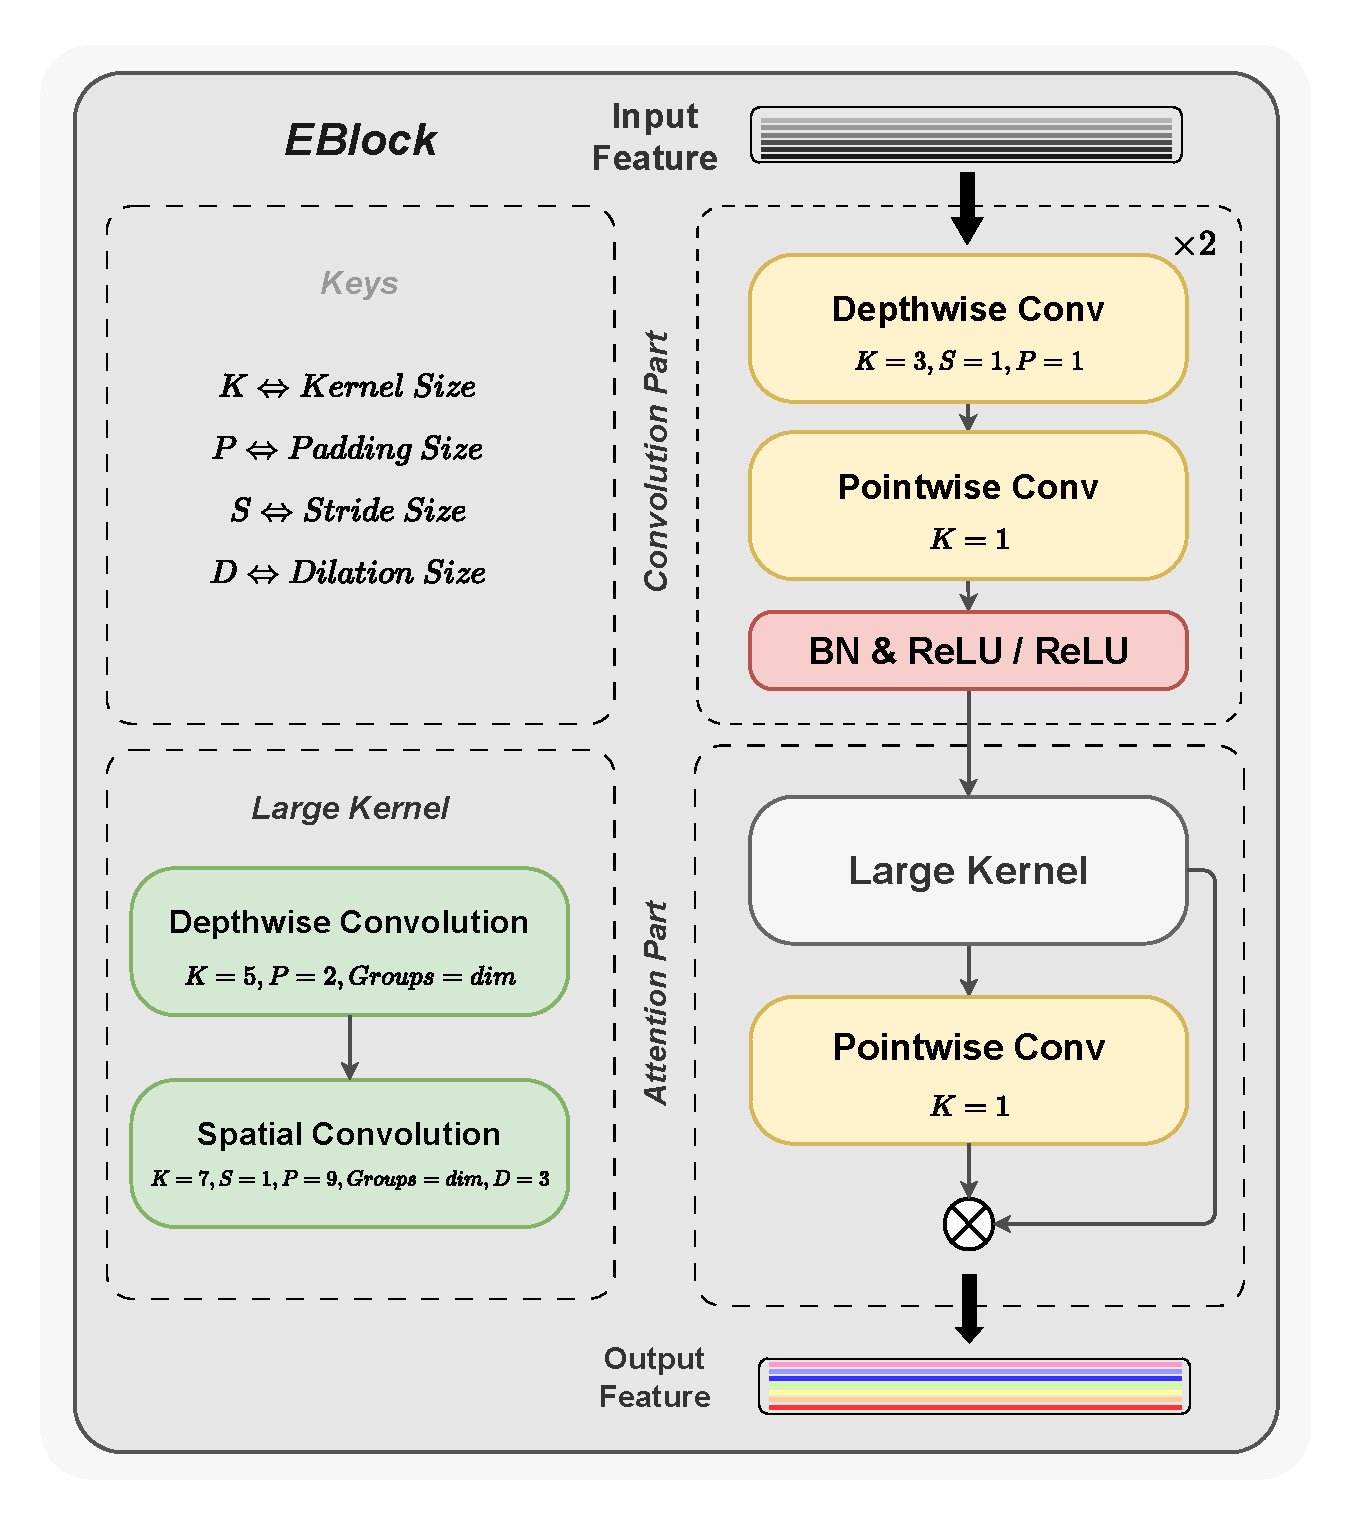
\includegraphics[height=0.6\textheight]{figure2.pdf}
    \caption{The architecture of \textbf{EBlock} and the components of convolution part and attention part}\label{fig2}
\end{figure}

% 介绍卷积部分的工作流程
The convolution part primarily comprises two consecutive layers of depthwise convolution, pointwise convolution, an activation function, and a batch normalization layer.
We configure the kernel size as \(3\times 3\), stride as 1, and padding as 1.
% 把下面两段精简一下到这一段内
Depthwise convolution processes each input channel independently, whereas traditional convolution spans all channels simultaneously.
It is a specialized convolution operation that performs convolutions independently within each input channel, which focuses on capturing local spatial features.
Pointwise convolution focuses on feature combination and transformation along the channel dimension.
It operates on each pixel of the input feature map, linearly combining features from different channels to generate new channel features with a \(1\times 1\) convolution kernel.
This sequence design significantly enhances the model's feature extraction capability while improving computational efficiency.

% 介绍通过深度可分离以及点卷积之后的的相关操作
Following the depthwise and pointwise convolution operations, we incorporate a subsequent layer combined with batch normalization and ReLU activation for the initial iteration.
This combination will employ only ReLU activation for the next subsequent iteration.
By utilizing EBlock, DLKUNet efficiently captures both spatial and semantic information and optimizes the parameter count by reducing computational overhead, this architecture ensures the model's effectiveness and performance in complex tasks.

% 开始用公式表达整个过程,让说明更加充分
Assuming the input feature map \(Z\in\mathbb{R}^{H\times W\times C}\), where \(H\) and \(W\) represent the height and width of the feature map,
and \(C\) denotes the number of channels, the convolution part can be formulated as follows

\begin{equation}
    Z_{l-1}' = \sigma_1 \left(BN\left(PointwiseConv\left(DepthwiseConv\left(Z_{l-1}\right)\right)\right)\right)
    \label{eq1}
\end{equation}

\begin{equation}
    Z_l = BN\left(PointwiseConv\left(DepthwiseConv\left(Z_{l-1}'\right)\right)\right)
    \label{eq2}
\end{equation}

where \(Z_{l-1}\) represents the feature tensor passed from the \(\left(L-1\right)\) layer, \(\sigma_1\) denotes the ReLU activation function, and BN refers to the batch normalization layer, which is used to standardize features.
In the \(L\) layer of the network, the input feature map \(Z_{l-1}\) is first processed by depthwise convolution, an operation that independently applies convolutions on each input channel.
The result is then passed through pointwise convolution, which facilitates the fusion of information across channels. 
The intermediate feature representation \(Z_{l-1}'\) is subsequently obtained through the combination of batch normalization and activation functions.
This intermediate representation is processed again using similar depthwise and pointwise convolutions, followed by batch normalization, resulting in the output feature map \(Z_{l}\).

% 开始介绍注意力部分的工作流程
The attention part consists of the large kernel module, the channel convolution module, and the Hadamard product operation.
We configure the kernel size as 5, padding as 2 and the number of groups equals the input dimension.
The attention part is designed to enhance the model's feature representation by capturing global contextual information and facilitating feature interaction across channels.
By increasing the size of the receptive field, the large kernel is capable of aggregating features from distant spatial regions, effectively incorporating more global context.
It helps the model better understand spatial relationships, making it more sensitive to subtle or complex features in the image.

% 介绍剩下来的相关模块
The output from the large kernel is processed through pointwise convolution to reduce the number of channels, thereby decreasing computational complexity while preserving key information.
The Hadamard product operation calculates inter-channel correlations to highlight important features while suppressing irrelevant or redundant information.
This design ensures that critical features receive higher priority within the channel dimension, improving the model's selective attention mechanism.
Additionally, the residual connection maintains the integrity of information, preventing feature degradation.

% 开始用公式表达整个过程,让说明更加充分
The attention module can be described using the following methodology

\begin{equation}
    Z_{LargeKernel} = PointwiseConv\left(SpatialConv\left(DepthwiseConv\left(Z_{l-1}\right)\right)\right)
\end{equation}

\begin{equation}
    Z_{l} = Z_{l-1} \otimes ChannelConv_{1\times 1}\left(Z_{LargeKernel}\right)
\end{equation}

% 简单解释一下公式
where \(Z_{l-1}\) represents the input feature map from the convolution part, and each channel is processed independently.
Spatial convolution is applied to expand the receptive field, capturing a broader range of contextual information.
Following this, pointwise convolution is employed to integrate the channel information, further strengthening the model's ability to capture global features.
The resulting feature map \(Z_{LargeKernel}\) is combined with the output from the \(1\times 1\) channel convolution by using a Hadamard product operation to enable inter-channel information interaction as \(Z_l\).


\subsection{DFB}\label{subsec3}

% 介绍一下DFB的主要组成部分
As shown in Figure \ref{fig3}, the Decoder Fusion Block consists of a fusion part, a convolution part, and an attention Part.

\begin{figure}[ht]
    \centering
    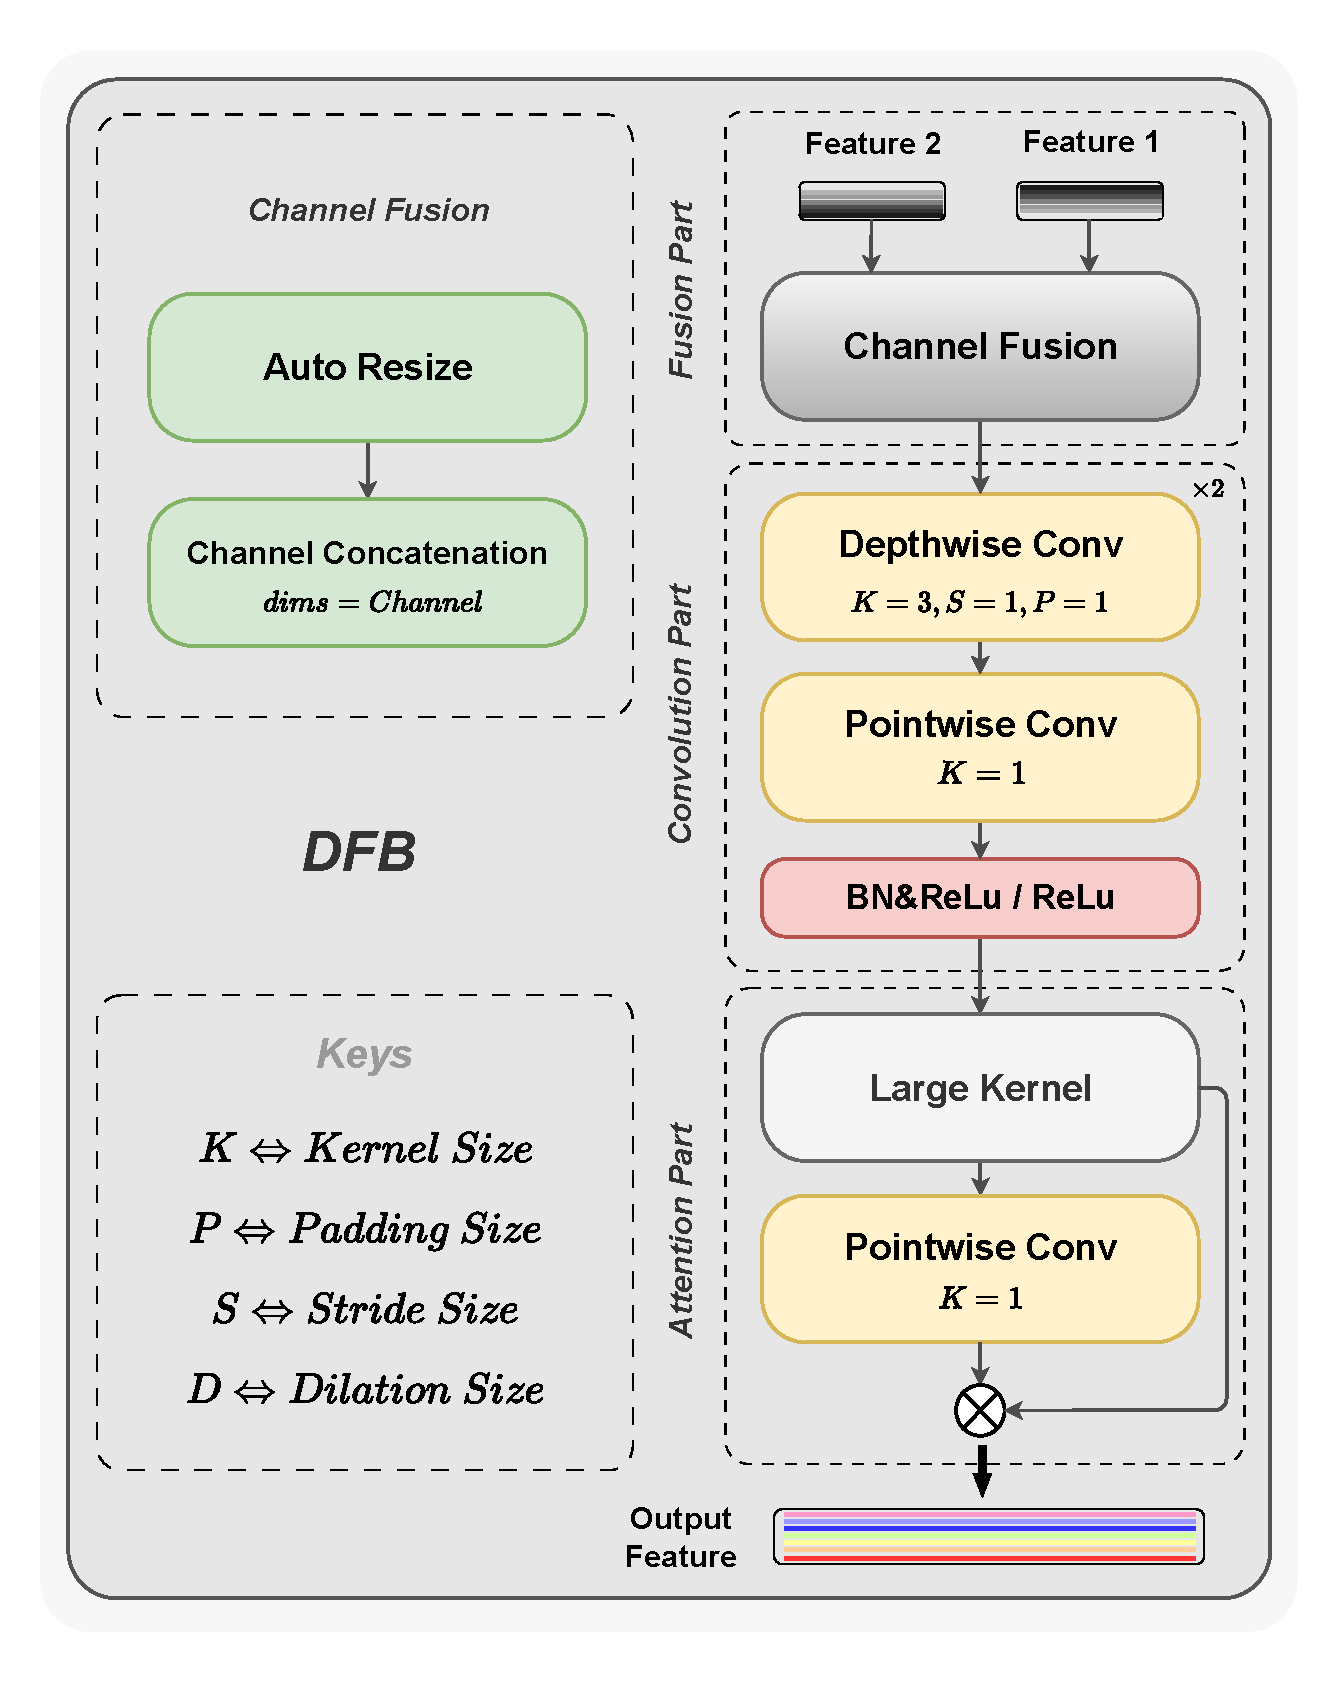
\includegraphics[height=0.6\textheight]{figure3.pdf}
    \caption{The architecture of \textbf{DFB} and its major components with working processes}\label{fig3}
\end{figure}

% 介绍channel fusion部分的工作原理
The fusion part primarily consists of an auto-resize component and a channel concatenation operation.
The auto-resize component is designed to resolve the height and width differences between the skip connection feature map and the decoder feature map.
To address these discrepancies, the decoder feature map is first upsampled to double its resolution, followed by zero-padding to match the dimensions of the skip connection feature map.
By applying appropriate upsampling and padding operations, the model ensures that feature maps from different paths and scales can be seamlessly merged.

% 介绍卷积部分和之前的EBlock是一样的
The convolution part and the attention part adopt a structure analogous to that of the encoder, facilitating close integration and synergy between the two.
It includes depthwise convolution, batch normalization, ReLU activation, and large kernel convolution, and further integrates features through pointwise convolution (with \(1\times 1\) kernel size).
This modular design enables the efficient processing of fused features, extracting more refined and high-quality feature information.

% 简短的总结
Through these computational modules, the decoder can effectively integrate the processed feature tensors, improving the network's feature representation.

\subsection{Architecture Variants}\label{subsec4}

% 介绍三种网络的不同的名称
We designed different network configurations as Figure \ref{fig4} and Figure \ref{fig1}.
These networks are named DLKUNet-S, DLKUNet-M, DLKUNet-L.
"S" denotes the smallest network, which is suitable for resource-constrained environments such as edge and mobile computing.
"M" represents the medium-sized network, striking a balance between computational cost and performance.
"L" indicates a larger parameter network in Figure \ref{fig1}, which offers superior segmentation performance compared to the smaller versions.

\begin{figure}[h]
    \centering
    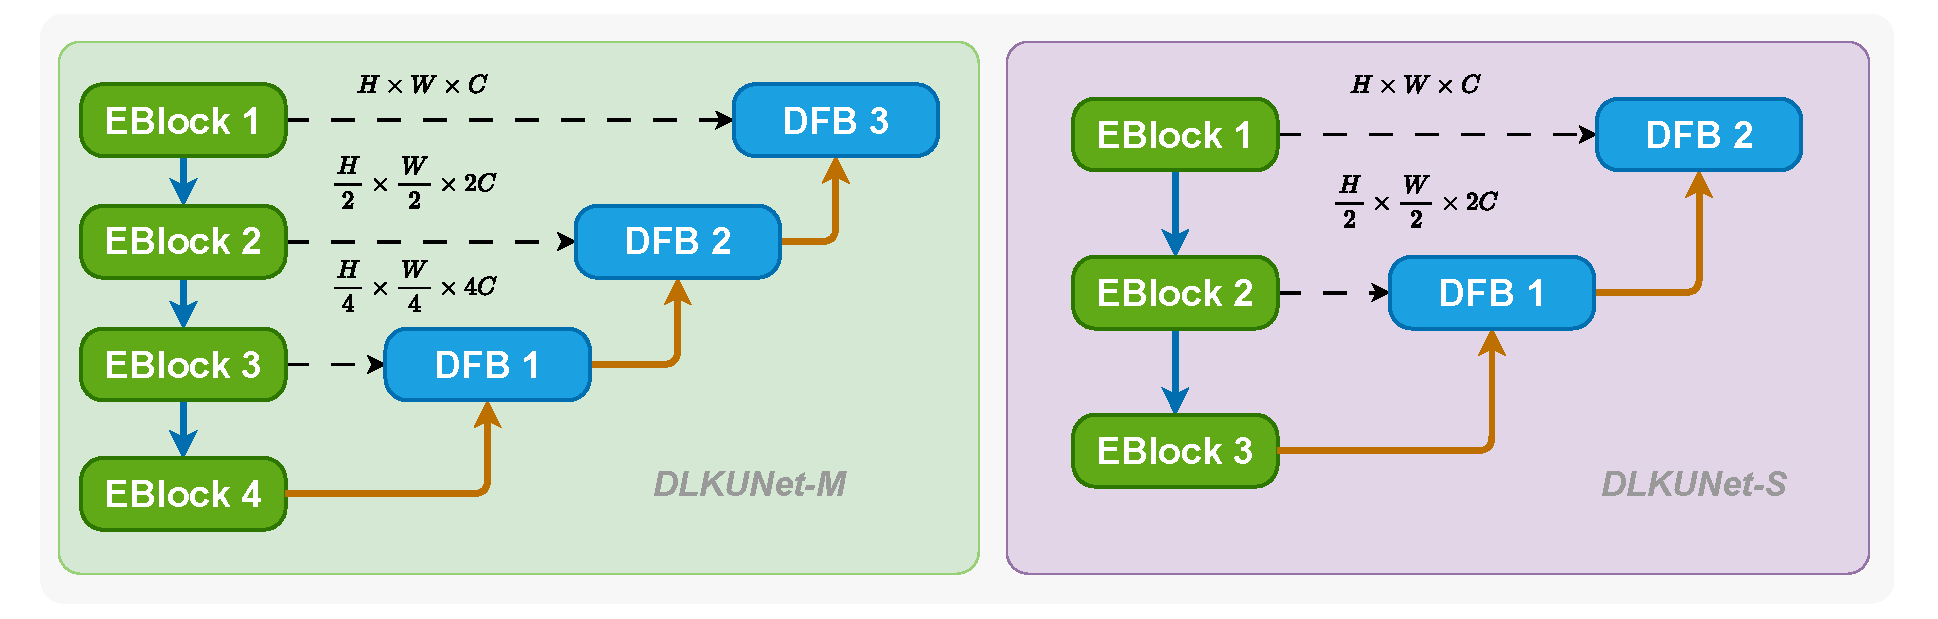
\includegraphics[width=\textwidth]{figure4.pdf}
    \caption{The architectural configurations of DLKUNet-M and DLKUNet-S}\label{fig4}
\end{figure}

% 介绍三种网络的不同配置
The configurations of the different DLKUNet models are summarized in Table \ref{tab1}.
Each model varies in terms of parameter count (Params), floating point operations (FLOPs) when input resolution is \(224\times 224\), the number of EBlock, the number of DFB, and the channel configuration for each skip connection (Channels Num).

DLKUNet-S is the smallest model, making it highly efficient for use in resource-constrained environments with only 1.13 million parameters and 15.95 GFLOPs.
It utilizes 3 encoder blocks and 2 decoder fusion blocks, and skip connection channels configured as \(C=96\).
DLKUNet-M is a medium-sized model, featuring 4.49 million parameters and 22.84 GFLOPs.
This model balances computational efficiency with performance and has 4 encoder blocks, and 3 decoder fusion blocks, with skip connection channels configured as \(C=96\).
DLKUNet-L is the largest model, with 17.7 million parameters and 29.64 GFLOPs.
It is suitable for scenarios where computational resources are less of a concern, and higher performance is desired.
DLKUNet-L includes 5 encoder blocks,4 decoder fusion blocks, and the channel configuration is \(C=96\).

% 简单的总结
These three models offer different trade-offs between computational complexity and feature extraction capability, enabling researchers and practitioners to select the appropriate model based on their specific resource limitations and performance requirements.
By providing different model sizes, DLKUNet is versatile and adaptable for a wide range of medical image segmentation tasks.

\begin{table}[h]
    \caption{Configurations of different DLKUNet models}\label{tab1}
    \centering
    \begin{tabular*}{\textwidth}{@{\extracolsep{\fill}} lccccc}
        \toprule
        Methods & Params (M) & FLOPs (G) & EBlock Num & DFB Num & Channels Num \\
        \midrule
        DLKUNet-S & 1.13 & 15.95 & 3 & 2 & \{96, 192\} \\
        DLKUNet-M & 4.49 & 22.84 & 4 & 3 & \{96, 192, 384\} \\
        DLKUNet-L & 17.70 & 29.64 & 5 & 4 & \{96, 192, 384, 768\} \\
        \bottomrule
    \end{tabular*}
\end{table}

\section{Experiments and Results}\label{sec4}

\subsection{Datasets}\label{subsec5}

\textbf{Multi-Organ Segmentation (Synapse) Dataset:}
% 介绍数据集
To validate the effectiveness of our method, we employed the widely recognized Synapse dataset \footnote{https://www.synapse.org/Synapse:syn3193805/wiki/217789}.
This dataset comprises 30 cases, with a total of 3,779 axial CT slices of the abdomen.
Each case contains between 85 and 198 slices, with a spatial resolution ranging from \(0.54\times 0.54\) to \(0.98\times 0.98 mm^2\) and pixel resolution of \(512\times 512\).
The slice thickness varies from 2.5 to 5.0 mm.
The dataset covers eight abdominal organs, including the aorta, gallbladder, spleen, left kidney, right kidney, liver, pancreas, and stomach.
In alignment with other related works \cite{cao2022swin,chen2021transunet}, we selected 18 cases from the Synapse dataset, totaling 2,211 longitudinal CT slices as the training dataset, with the remaining 12 cases used for testing.

\textbf{Automated Cardiac Diagnosis Challenge (ACDC) Dataset:}
The ACDC dataset \footnote{https://www.creatis.insa-lyon.fr/Challenge/acdc/} comprises MRI images of cardiac anatomy from different patients, with annotations for the left ventricle (LV), right ventricle (RV), and myocardium (MYO).
For the ACDC dataset, we preprocessed the dataset and used 70 training samples, with a total of 1,304 slices for training, and 20 test samples, with 40 slices for testing\cite{cao2022swin,chen2021transunet}.

\subsection{Evaluation Metrics}

\textbf{The Dice Similarity Coefficient (DSC):}
% 介绍评估指标DSC
DSC is a metric used to measure the similarity between two samples, ranging from \(\left[0,1\right]\), where 1 represents perfect overlap and 0 represents no overlap\cite{sudre2017generalised,cao2022swin}.
Let \(A\) represent the predicted segmentation result, and \(B\) represent the corresponding ground truth region.
Higher DSC indicates better performance in medical image segmentation.
The DSC is given as

\begin{equation}
    DSC\left(A,B\right) = \frac{2\times\left|A\cap B\right|}{\left|A\right|+\left|B\right|}\label{eq11}
\end{equation}

\textbf{The 95\% Hausdorff Distance (HD95):}
% 介绍评估指标HD95
HD is a metric that quantifies the similarity between two sets by measuring the maximum distance between their boundaries\cite{huttenlocher1993comparing,chen2021transunet}.
HD95 refers to the \(95th\) percentile of the Hausdorff distance.
Here, \(d\left( s,t \right)\) represents the Euclidean distance between point \(s\) and \(t\), while \(sup\) and \(inf\) denote the supremum and infimum respectively.
Lower HD95 indicates better performance in medical image segmentation.
The HD95 is given as

\begin{equation}
    HD95(S, T) = Percentile_{95}\left( \left\{ \inf_{t \in T} d(s, t) \mid s \in S \right\} \cup \left\{ \inf_{s \in S} d(t, s) \mid t \in T \right\} \right) \label{eq12}
\end{equation}

\subsection{Implementation details}\label{subsec6}

% 介绍训练的具体参数
We conducted model training in the PyTorch 2.4.1 environment, using Python version 3.12.4, and the GPU hardware configuration is Nvidia A800.
In the training process, no third-party datasets were used for pretraining.
We employed the Adam optimizer, with weight decay coefficient set to \(1e-5\), input image size of \(224\times 224\), and initial learning rate of \(1e-3\), and after 200 epochs, the learning rate was adjusted to \(1e-5\).
Also, a dynamic learning rate adjustment strategy was applied, reducing the learning rate by 90\% every 20 epochs, optimizing the model's convergence speed and final performance at different stages of training.	

% 介绍数据强化的工作
To improve the network's robustness, we applied data augmentation techniques to the training datasets.
For both the Synapse and ACDC datasets, we employed data augmentation strategies involving random flipping and random \(90^{\circ}\) rotation, each applied with a probability of 50\%.
These techniques effectively enhanced the network's robustness in segmentation tasks, ensuring high accuracy and stability when handling various image transformations and variations.

\subsection{Training Strategies}

% 介绍其他方法常用的Loss函数以及训练策略
To balance both the boundary features and accurate segmentation of target regions, the following composite loss function is commonly used to optimize the segmentation performance in medical image segmentation.

\begin{equation}
    OrdinaryLoss = DiceLoss + CELoss\label{eq13}
\end{equation}

In the aforementioned strategy for calculating the loss function, DiceLoss refers to the Dice Similarity Coefficient loss function, which is computed as

\begin{equation}
    DiceLoss = 1-\frac{2\times\left|P\cap G\right|+\epsilon}{\left|P\right|+\left|G\right|+\epsilon}\label{eq14}
\end{equation}

where \(P\) represents the predicted segmentation region, \(G\) represents the ground truth region, \(\left|P\cap G\right|\) denotes the intersection between the predicted and ground truth areas,
and \(\left|P\right|\) and \(\left|G\right|\) represent the number of voxels in the predicted and ground truth areas, respectively.
\(\epsilon\) is used to avoid division by zero.

CELoss represents Cross-Entropy Loss, and for multiclass classification problems like the Synapse or ACDC dataset, it can be expressed as

\begin{equation}
    CELoss = -\sum_{i=1}^{C}{G_i\log{\left(P_i\right)}}\label{eq15}
\end{equation}

where \(C\) denotes the number of classes, \(P_i\) represents the predicted probability for the class, and \(G_i\) is the true label for the class.

% 介绍过去常用方法的好处以及缺点
Compared with using DiceLoss or CELoss individually, this composite method more effectively balances the learning of edge features and central regions.
DiceLoss focuses on optimizing the overlap ratio, ensuring that the network captures the global contour of the target.
In contrast, CELoss focuses on pixel-level classification, which is particularly beneficial for identifying small or challenging regions in imbalanced datasets.
This combination improves both the segmentation accuracy and robustness of the model.
However, when handling regions with varying complexities, such as intricate boundaries versus simpler central areas, the convergence rate of the loss function may differ between these regions.
This discrepancy can lead to situations where one part of the data, such as the central regions, has already been well-fitted, while the complex boundaries continue to converge at a much slower rate,
ultimately affecting the overall segmentation performance.

% 介绍自己的训练策略
To improve the fitting of the loss function, we applied two specific dynamic loss function strategies.

\textbf{Phase-based Loss Strategy:}
% 介绍自己的第一个训练策略
This strategy adjusts the composition ratio of loss functions and the learning rate based on different stages of the training process.
In the early stages of training, global and local features are equally important, so the weights of CELoss and DiceLoss are set equally.
In later stages, to refine the segmentation results, the weight of DiceLoss is increased.
Simultaneously, the learning rate is adjusted according to the training phase to ensure stable convergence and optimal performance.

\textbf{Dynamic Loss Strategy:}
% 介绍自己的第二个训练策略
This strategy automatically adjusts the ratio between DiceLoss and CELoss during training and dynamically modifies the loss weights based on predefined rules.
For example, we observed that the model fits global features faster than local features in the ACDC dataset.
By applying this method, the model can flexibly adjust the weighting of the loss functions, improving training efficiency and segmentation accuracy.

Both the Phase-based and Dynamic Loss Strategy can be expressed as

\begin{equation}
    Loss = \alpha\times DiceLoss + \beta\times CELoss\label{eq16}
\end{equation}

when using a \textbf{Phase-based Loss} Strategy, set \(\alpha\) and \(\beta\) as

\begin{equation}
    (\alpha, \beta) =
    \begin{cases}
        (0.6, 0.4), & \text{epochs \(\in\) } [1, 200] \\
        (0.7, 0.3), & \text{epochs \(\in\) } (200, 400]\label{eq17}
    \end{cases}
\end{equation}

when using \textbf{Dynamic Loss} function, set as

\begin{equation}
    \alpha = A + \left(1-A\right)\times\left(1-\frac{1}{1+e^{-k\left(x-x_0\right)}}\left(epoch\right)\right)
\end{equation}

\begin{equation}
    \beta = 1 + \left(B-1\right)\times\left(1-\frac{1}{1+e^{-k\left(x-x_0\right)}}\left(epoch\right)\right)
\end{equation}

here \(k\) denotes the slope of the curve, and \(x_0\) represents the midpoint offset value, which is typically set to \(0.5\times epoch\).
\(A\) and \(B\) usually set as \(0.3\) and \(0.7\).

% 介绍自己的训练策略在Synapse数据集上的表现
In the Synapse segmentation task, Figure \ref{fig5} illustrates the DSC performance during training when using the DLKUNet-L with OrdinaryLoss and Phase-Based Loss (ours).
The x-axis represents the number of training epochs, and the y-axis shows the DSC on the test set. 
As shown in the figure, the model trained with Phase-Based Loss (red curve) exhibited better convergence and higher segmentation accuracy throughout the training process.
In contrast, the model with OrdinaryLoss (blue curve) showed slower convergence in the early training stages and exhibited greater fluctuation in the later stages.
The Phase-Based Loss strategy significantly outperformed the OrdinaryLoss strategy in the Synapse dataset, improving segmentation capability and accelerating convergence.

\begin{figure}[ht]
    \centering
    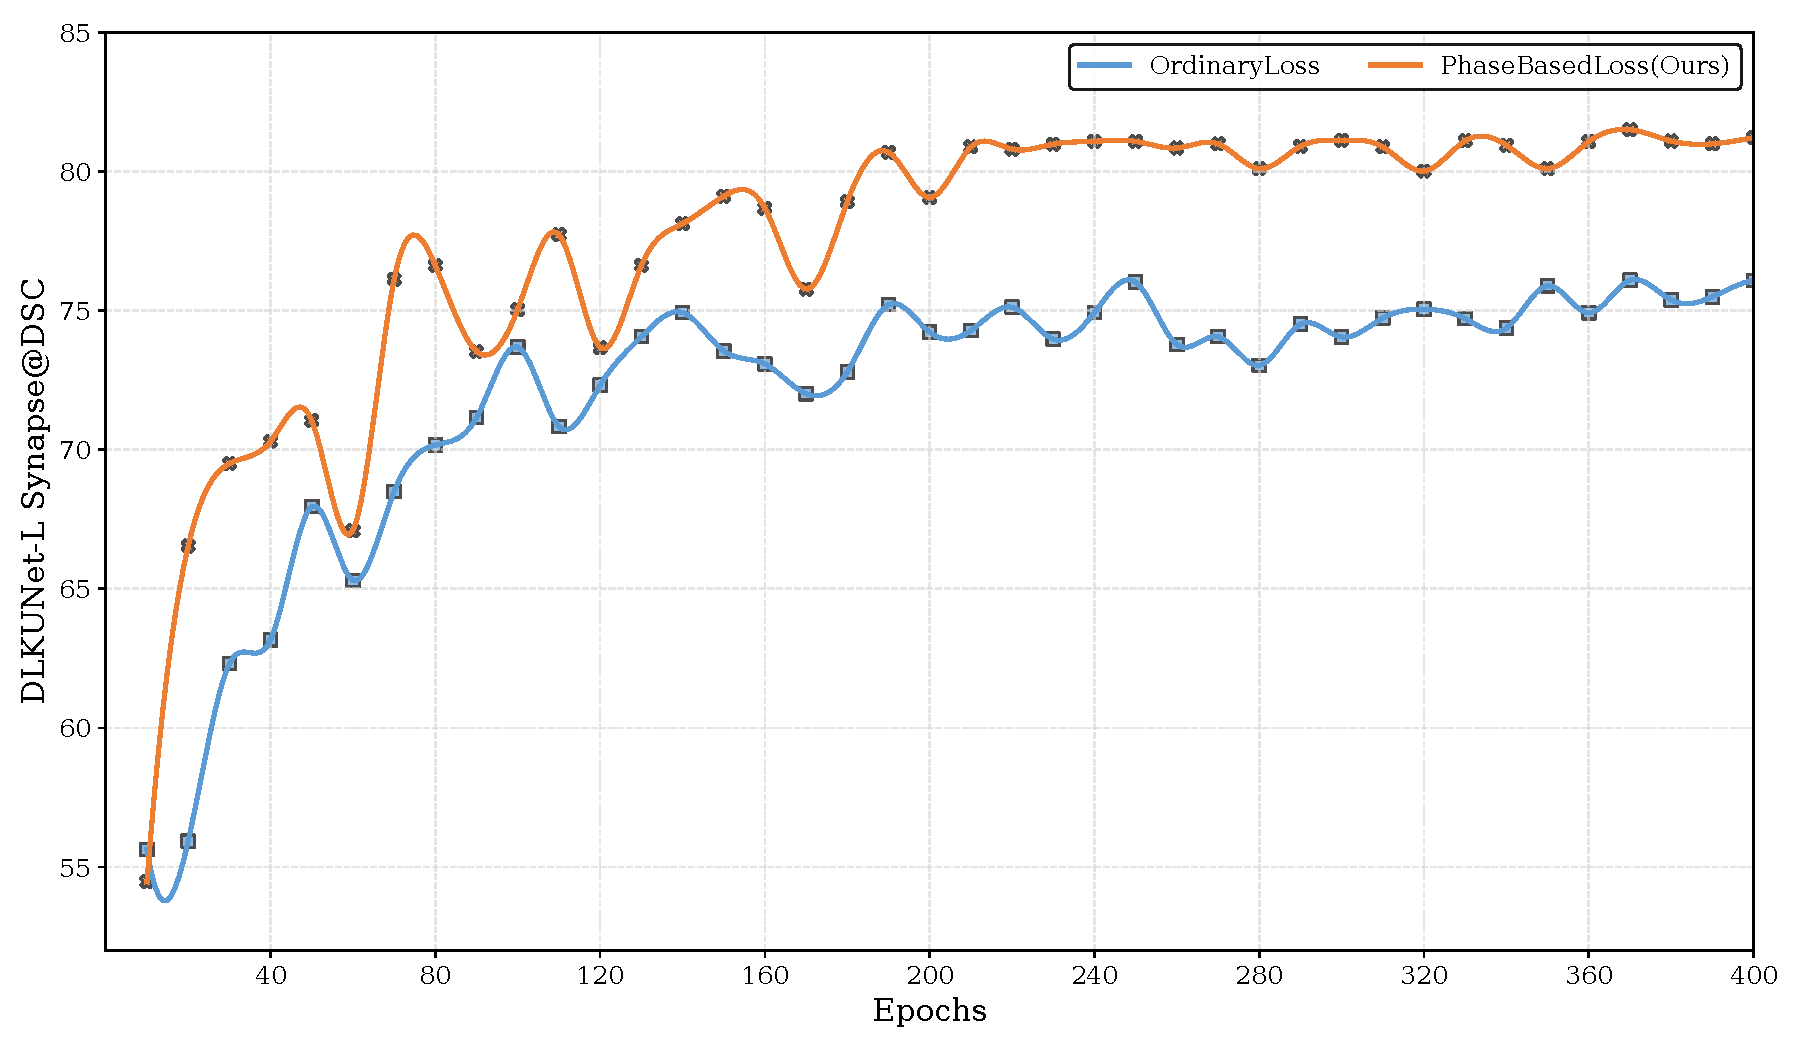
\includegraphics[width=\textwidth]{figure5.pdf}
    \caption{DSC scores obtained from segmenting the Synapse dataset using DLKUNet-L under different loss functions.
    The blue line represents the OrdinaryLoss method, while the red line denotes the Phase-Based Loss method.}\label{fig5}
\end{figure}

% 介绍自己的训练策略在ACDC数据集上的额
Similarly, in the ACDC dataset, Figure \ref{fig6} shows the scoring performance of PhaseBasedLoss and DynamicLoss strategies during training when using DLKUNet-L.
The x-axis represents the number of training epochs.
As shown in the figure, the red curve, which represents the Dynamic Loss strategy that continuously adjusts the loss function in real-time, demonstrates faster convergence and a more stable DSC compared to the blue curve representing PhaseBasedLoss.
\begin{figure}[ht]
    \centering
    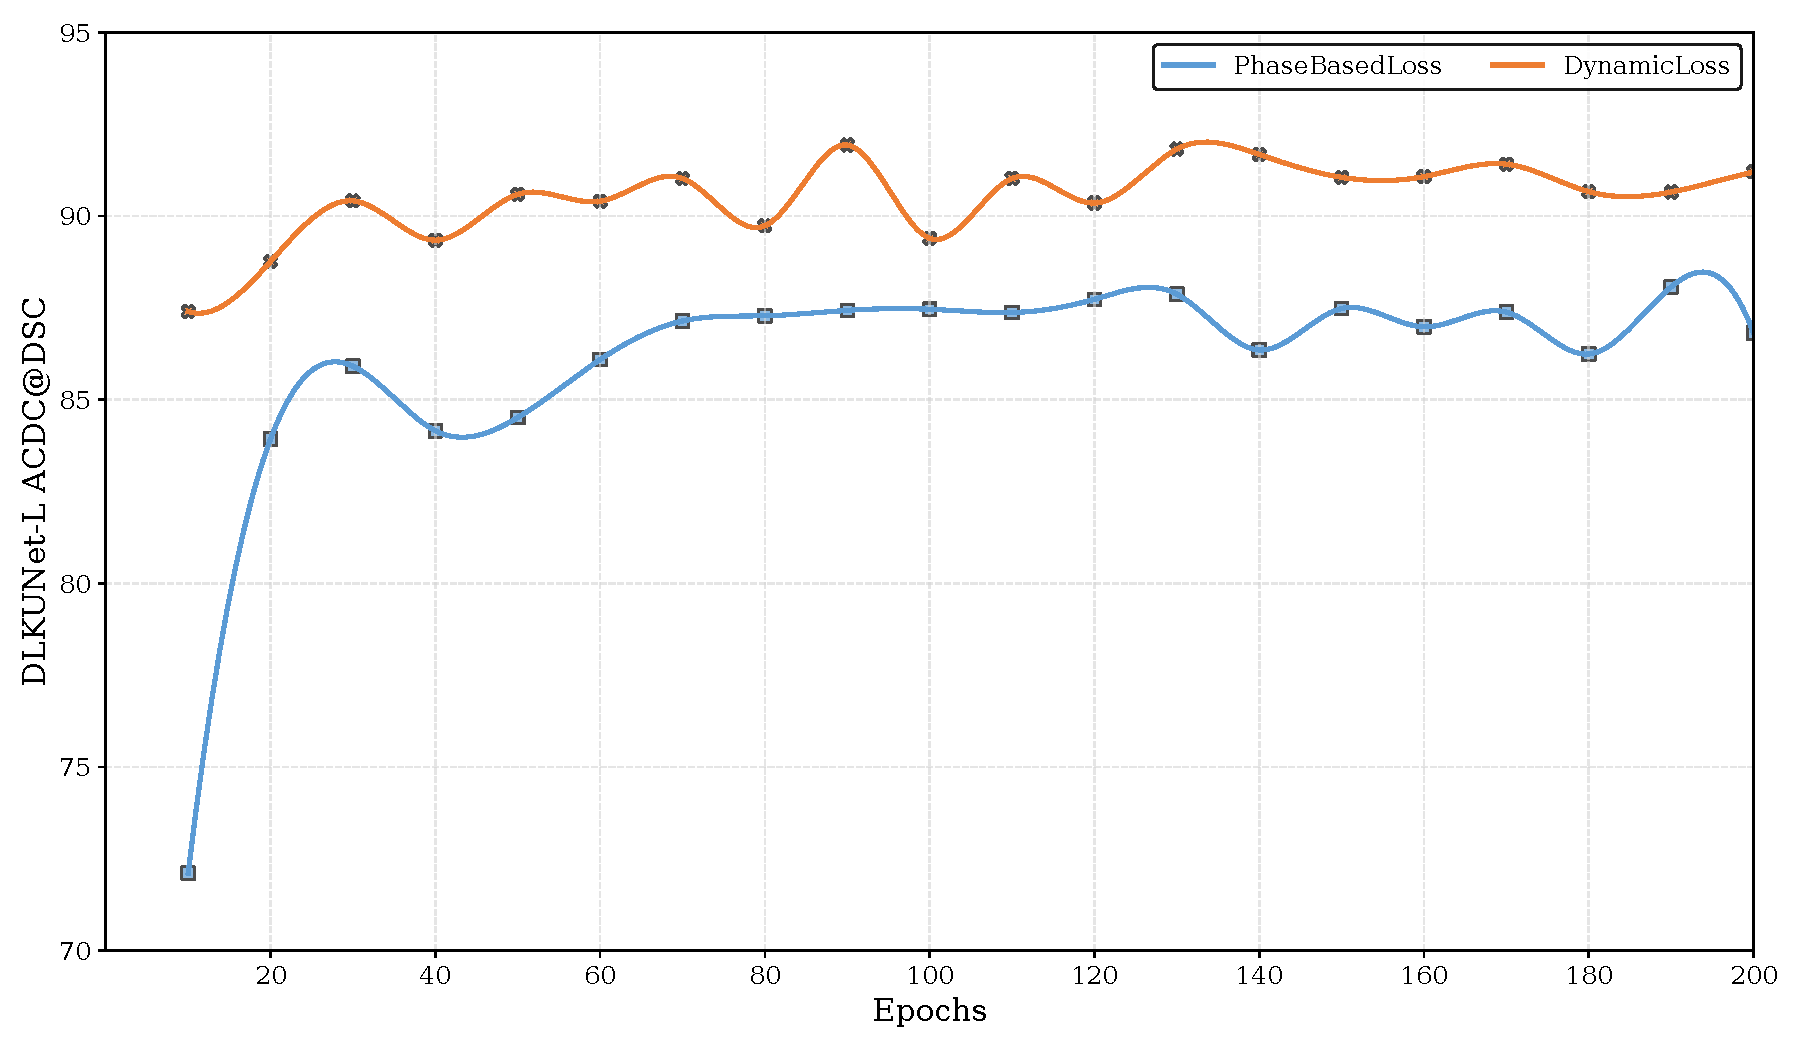
\includegraphics[width=\textwidth]{figure6.pdf}
    \caption{DSC scores obtained from segmenting the ACDC dataset using DLKUNet-L under different loss functions.
    The blue line represents the use of the Phase-Based Loss strategy, while the red line denotes the use of the Dynamic Loss strategy.}\label{fig6}
\end{figure}

% 最终得出的结论
From these two sets of experimental results, it can be concluded that the Phase-Based Loss strategy performs better in handling the complex Synapse multi-organ segmentation task,
while the Dynamic Loss strategy is more advantageous in the ACDC segmentation task.
These strategies significantly improve the model's convergence speed and final performance.

\subsection{Experiment Results}\label{subsec7}

% 介绍Synapse数据集上虞其他模型之间的比较
As shown in Table \ref{tab2} and Figure \ref{fig7}, we conducted a comparison of our method against other approaches on the Synapse segmentation task.
We evaluate the segmentation performance on eight organs and analyze the parameter count and computational complexity of each method.

\begin{sidewaystable}
    \centering
    \caption{Comparative results of various methods in the Synapse segmentation task.
    The parameter count is measured in Million (M), and FLOPs are calculated in Gigaflops (G).
    Higher DSC indicates better performance, while lower HD95 indicates better performance.
    Evaluation on Aorta(Aor), Gallbladder(Gal), Left Kidney(Kid(L)), Right Kidney(Kid(R)), Liver(Liv), Pancreas(Pan), Spleen(Spl), Stomach(Sto)
    \textcolor{red}{Red} highlights the best results, while \textcolor{blue}{Blue} indicates the second-best results.}
    \label{tab2}
    \begin{tabular*}{\textwidth}{@{\extracolsep{\fill}}lcccccccccccc}
        \toprule
        \textbf{Method} & \textbf{Params(M)} & \textbf{FLOPs(G)} & \textbf{DSC} & \textbf{HD95} & \textbf{Aor} & \textbf{Gal} & \textbf{Kid(L)} & \textbf{Kid(R)} & \textbf{Liv} & \textbf{Pan} & \textbf{Spl} & \textbf{Sto} \\
        \midrule
        R50 U-Net\cite{chen2021transunet} & 147.80 & 41.09 & 74.68 & 36.87 & 87.74 & 63.66 & 80.60 & 78.19 & 93.74 & 56.90 & 85.87 & 74.16 \\
        U-Net\cite{ronneberger2015u} & 34.52  & 65.52 & 76.85 & 39.7  & 89.07 & 69.37 & 77.77 & 68.60 & 93.43 & 53.98 & 86.67 & 75.58 \\
        Att-U-Net\cite{oktay2018attention} & 34.87 & 66.63 & 77.77 & 36.2 & \textcolor{red}{89.55} & \textcolor{blue}{68.88} & 77.98 & 71.11 & 93.5 & 58.04 & 87.30 & 75.75 \\
        TransUNet\cite{chen2021transunet}  & 96.07  & 88.91 & 77.48 & 32.69 & 87.23 & 63.16 & 81.87 & 77.02 & \textcolor{blue}{94.09} & 55.86 & 85.08 & 75.62 \\
        Swin-Unet\cite{cao2022swin}  & 27.17  & \textbf{6.16}  & 79.13 & 21.55 & 85.47 & 66.53 & 83.28 & 79.61 & \textcolor{red}{94.29} & 56.58 & 90.66 & \textcolor{blue}{76.6} \\
        \midrule
        DLKUNet-S & \textbf{1.13} & 15.95 & 79.74 & 28.95 & 87.46 & 66.27 & 84.15 & 76.06 & 92.74 & \textcolor{red}{64.72} & 90.38 & 76.17 \\
        DLKUNet-M & 4.49 & 22.84 & 80.82 & 22.78 & \textcolor{blue}{88.14} & \textcolor{red}{72.39} & \textcolor{blue}{85.20} & \textcolor{blue}{81.13} & 92.88 & 60.46 & \textcolor{blue}{90.79} & 75.54 \\
        DLKUNet-L & 17.70 & 29.64 & \textbf{81.21} & \textbf{13.89} & 87.39 & 67.4 & \textcolor{red}{87.64} & \textcolor{red}{83.47} & 92.45 & 63.44 & \textcolor{blue}{90.99} & \textcolor{red}{76.92} \\
        \bottomrule
    \end{tabular*}
\end{sidewaystable}

% Synapse数据的可视化
\begin{figure}[h]
    \centering
    \includegraphics[width=\textwidth]{figure7.pdf}
    \caption{Visualization results obtained using different methods on the Synapse dataset.}\label{fig7}
\end{figure}

% 介绍三个模型与Swin-Unet模型在DSC数值上的关系
Although Swin-Unet \cite{cao2022swin} and U-Net \cite{ronneberger2015u} utilize similar U-shaped hierarchical designs that combine encoder and decoder modules to enhance feature extraction,
the DLKUNet architecture demonstrates superior segmentation performance across multiple organs.
DLKUNet-L achieves a 12.12\% improvement in DSC score compared to Swin-Unet for pancreas segmentation, while maintaining comparable performance in liver segmentation.
Additionally, it demonstrates approximately 2\% improvement in DSC score for other organs \cite{cao2022swin}.
DLKUNet-M also demonstrates significant advantages, achieving the highest score in gallbladder segmentation, it represents an 8.8\% improvement over Swin-Unet.
Even the smallest model outperforms Swin-Unet, achieving a DSC score of 79.74 compared to the Swin-Unet score of 79.13.

% 介绍三个模型与Swin-Unet模型在HD95数值上的关系
Our method excels in the DSC score, and also it shows superior performance in measuring the quality of segmentation boundaries.
DLKUNet-L models outperformes Swin-Unet \cite{cao2022swin} in HD95, with improving boundary precision by 35\%.
This demonstrates the superior ability of our model in edge detection and fine feature extraction.

% 模型的参数量与其他模型进行比较
In addition to achieving outstanding segmentation results, our method also demonstrates significant advantages in terms of parameter efficiency.
The DLKUNet-S uses only 4.1\% of the parameters of Swin-Unet \cite{cao2022swin}, and achieves a 0.7\% higher DSC score.
The DLKUNet-M uses 16.52\% of the parameters of Swin-Unet and achieves a 2.1\% higher DSC score.
The DLKUNet-L, utilizing 65\% of Swin-Unet parameters, surpasses it by 2.6\% in the DSC score.
Compared to traditional convolutional models such as R50 U-Net \cite{chen2021transunet}, our improvement is even more notable, requiring less than 1\% of the parameter count.

% 在ACDC数据集上进行比较DSC性能以及HD95能力
Similar to the segmentation task on the Synapse dataset, we also evaluated our method on the ACDC dataset, using the DSC as the evaluation metric.
As shown in Table \ref{tab3} and Figure \ref{fig8}, DLKUNet-L achieves a DSC score of 91.93, surpassing Swin-Unet \cite{cao2022swin} by 2.14\% while using only 65\% of its parameter count.
Moreover, the DLKUNet-M achieves a DSC score of 91.74 with a parameter count of 4.49M, this demonstrates excellent efficiency and segmentation performance.
Although the DLKUNet-S has a parameter count of only 1.13M, it still achieves a DSC score of 91.71, surpassing Swin-Unet.

\begin{table}[h]
    \centering
    \caption{Comparison of results for the ACDC task using different methods in terms of parameters (M) and DSC.
    Higher DSC scores indicate better segmentation performance.}
    \label{tab3}
    \begin{tabular*}{\textwidth}{@{\extracolsep{\fill}}lccccc}
        \toprule
        \textbf{Method} & \textbf{Params (M)} &  \textbf{DSC} & \textbf{RV} & \textbf{Myo} & \textbf{LV} \\
        \midrule
        R50 U-Net\cite{ronneberger2015u}  & 147.80 & 87.55 & 87.1 & 80.63 & 94.92 \\
        R50 Att-U-Net\cite{oktay2018attention}  & 34.87  & 86.75 & 87.58 & 79.20 & 93.47 \\
        R50 ViT\cite{dosovitskiy2020image}  & 97.96 & 87.57 & 86.07 & 81.88 & 94.75 \\
        TransUNet\cite{chen2021transunet}  & 96.07  & 89.71 & 88.86 & 84.53 & 95.73 \\
        Swin-Unet\cite{cao2022swin}  & 27.17  & 90 & 88.55 & 85.62 & 95.83 \\
        \midrule
        DLKUNet-S  & \textbf{1.13}  & 91.71 & \textbf{89.82} & 89.56 & 95.75 \\
        DLKUNet-M  & 4.49   & 91.74 & 89.48 & 89.94 & 95.81 \\
        DLKUNet-L  & 17.70  & \textbf{91.93} & 89.52 & \textbf{90.19} & \textbf{96.09} \\
        \bottomrule
    \end{tabular*}
\end{table}

\begin{figure}[h]
    \centering
    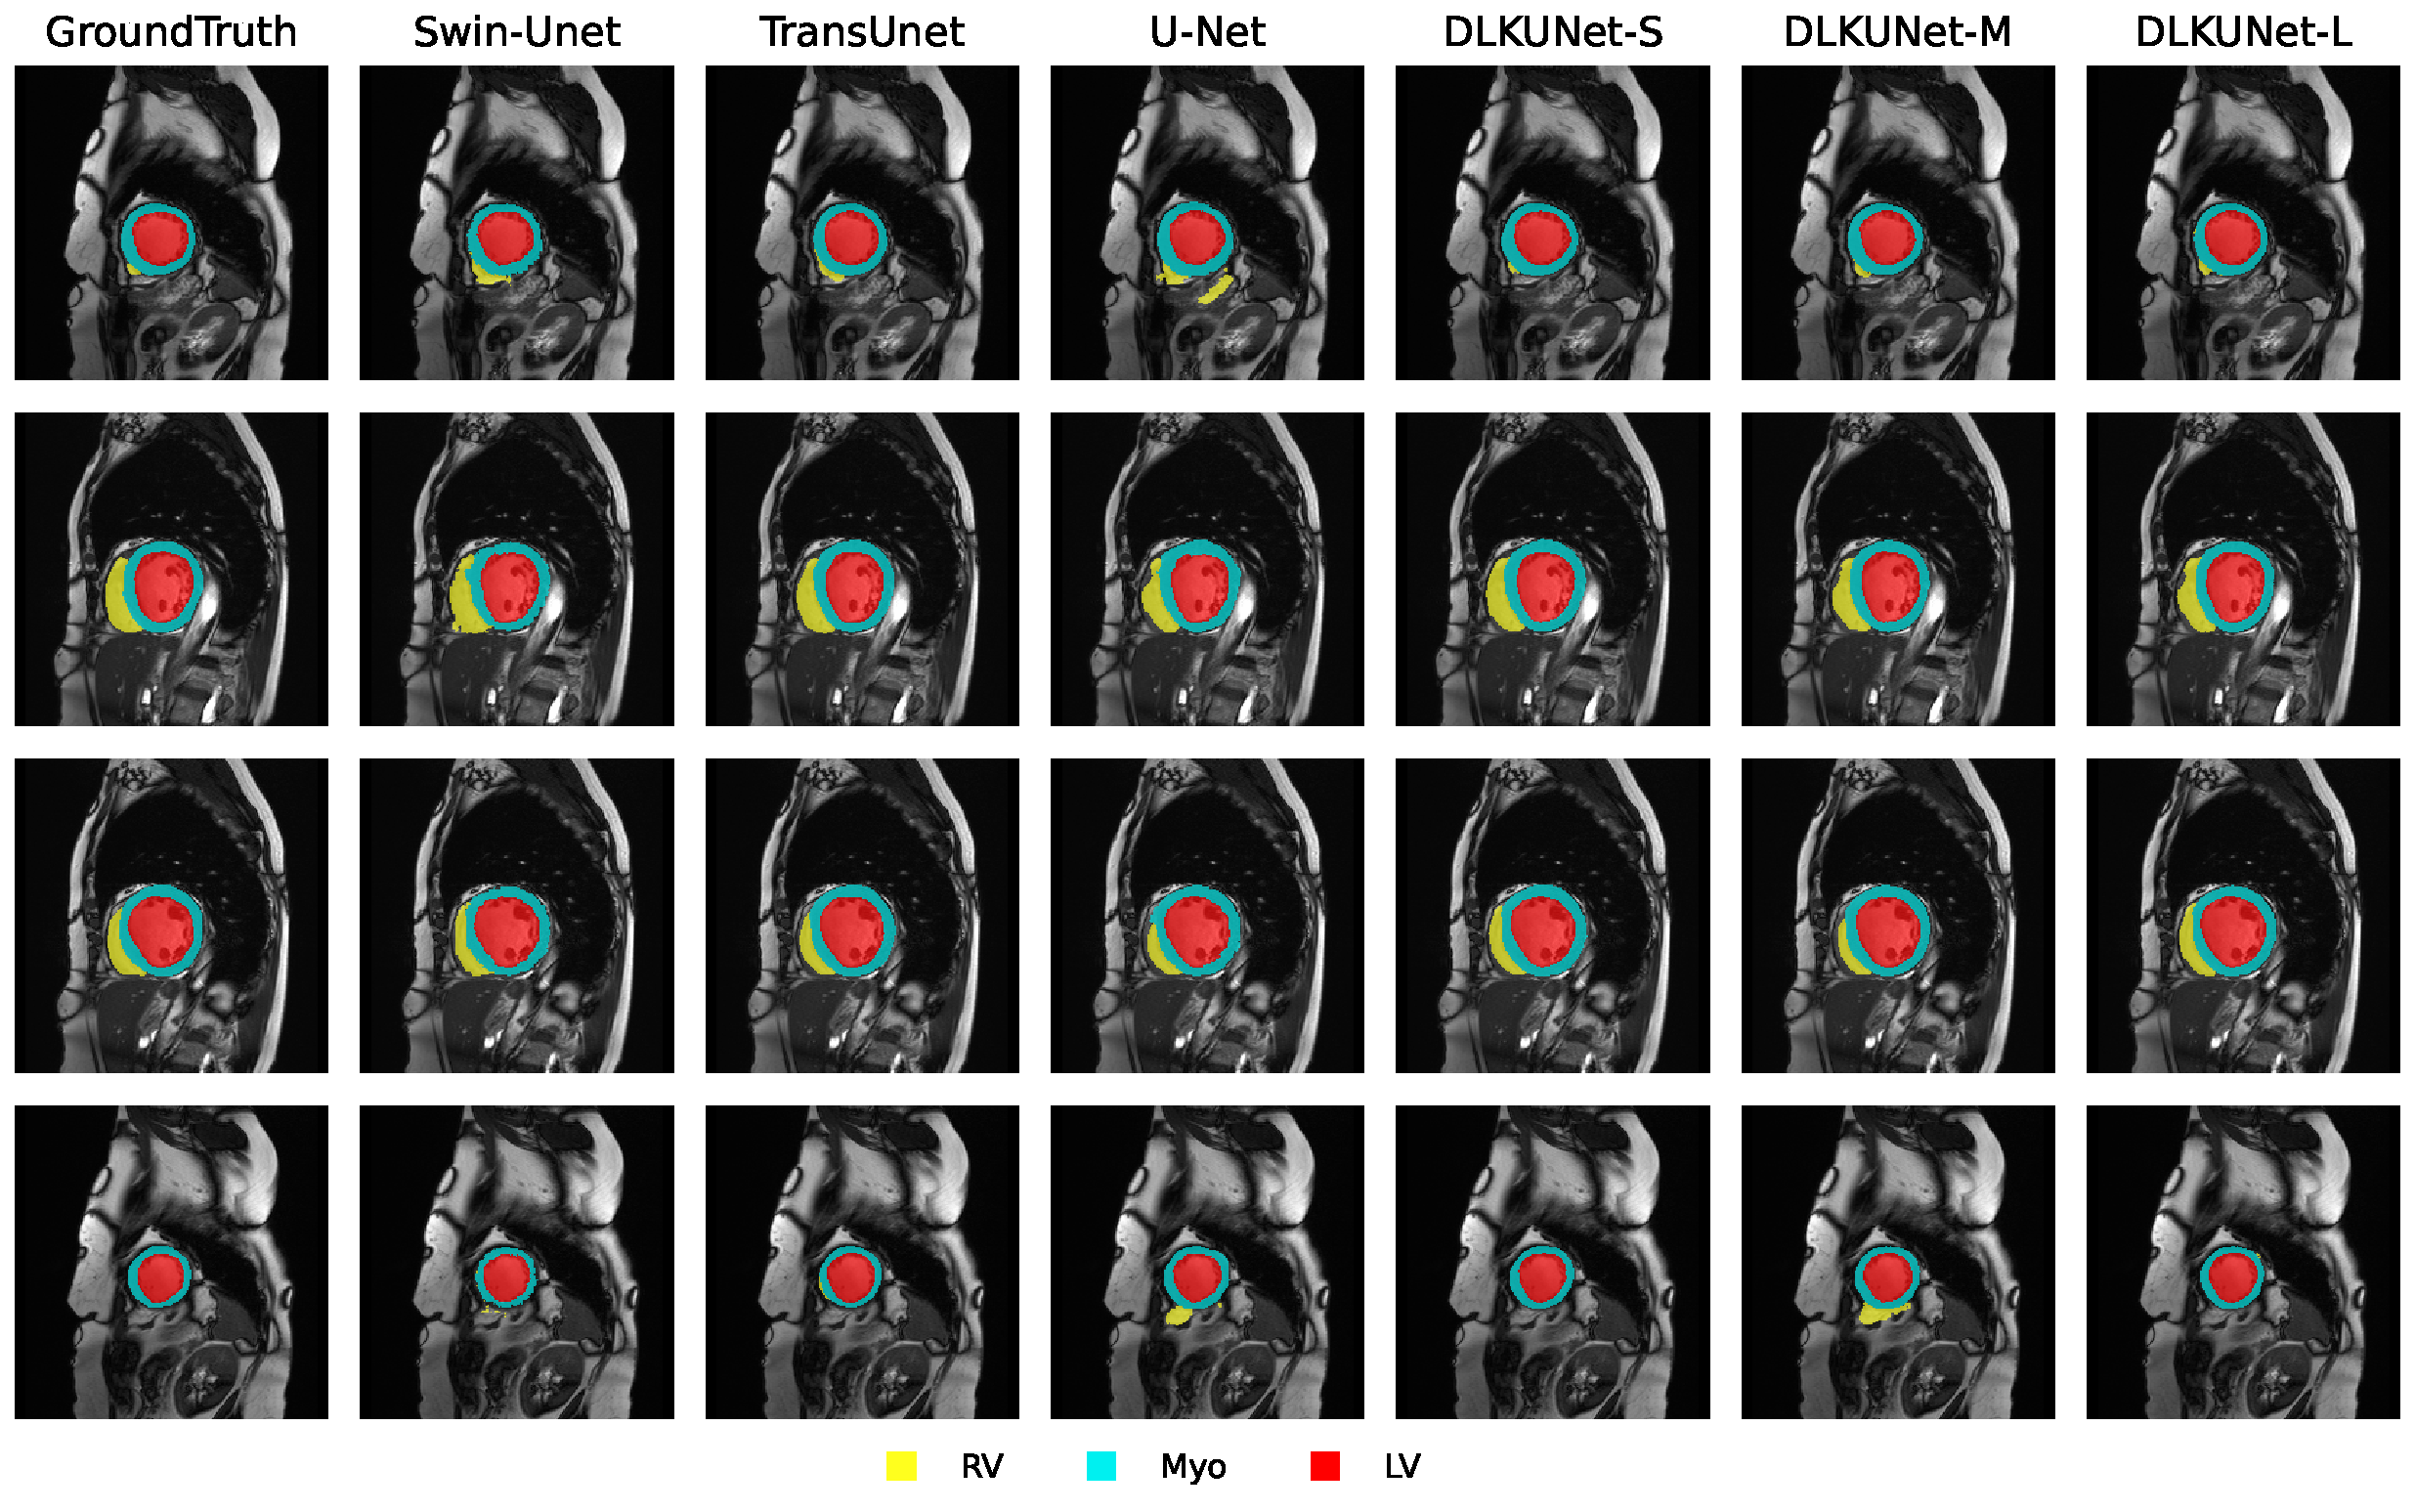
\includegraphics[width=\textwidth]{figure8.pdf}
    \caption{Segmentation results obtained using different methods on the ACDC task.}\label{fig8}
\end{figure}

% 简单的总结
Our method demonstrates outstanding generalization capabilities and robustness through testing on the Synapse and ACDC datasets,
maintaining excellent performance across various medical image segmentation tasks.

\section{Ablation Study} \label{sec5}

% 介绍消融实验
To further investigate the factors influencing network performance, we conducted ablation experiments on the Synapse dataset.

\textbf{Effect of Channels Count:}
% 介绍通道数消融实验的整体
Figure \ref{fig9} presents an ablation study examining the effects of varying skip connection settings on the performance of the DLKUNet architecture.
Specifically, the experiment evaluates DLKUNet-S, DLKUNet-M, and DLKUNet-L model configurations, each employing three different configurations of channel sizes.

% 介绍具体的实验参数配置以及图像中的意思
% 下面的内容需要改一下,现在没有C1,C2了
For the small model, three configurations were tested with channel settings of $C$ = 64, 96, 128 in the y-axis.
Similarly, the medium model and large model employ skip connections with channel configurations of $C$ = 64, 96, 128.
In total, nine model configurations were tested, producing eighteen experimental results, as represented in the heatmaps.

% 介绍实验的结果
We conducted DSC score and HD95 comparisons on the Synapse dataset for DLKUNet-S, DLKUNet-M, and DLKUNet-L model configurations, and the input image size is \(224\times 224\).
The experimental results show significant differences in segmentation performance across different channel counts and model sizes, as shown in Figure \ref{fig9}.
When the channel count is 96, the model achieved the best balance between the DSC score and HD95, especially in the DLKUNet-L model, where it achieves a DSC score of 81.21 and maintains good boundary precision \((13.89mm)\).

\begin{figure}[h]
    \centering
    \begin{subfigure}[b]{0.49\textwidth}
        \centering
        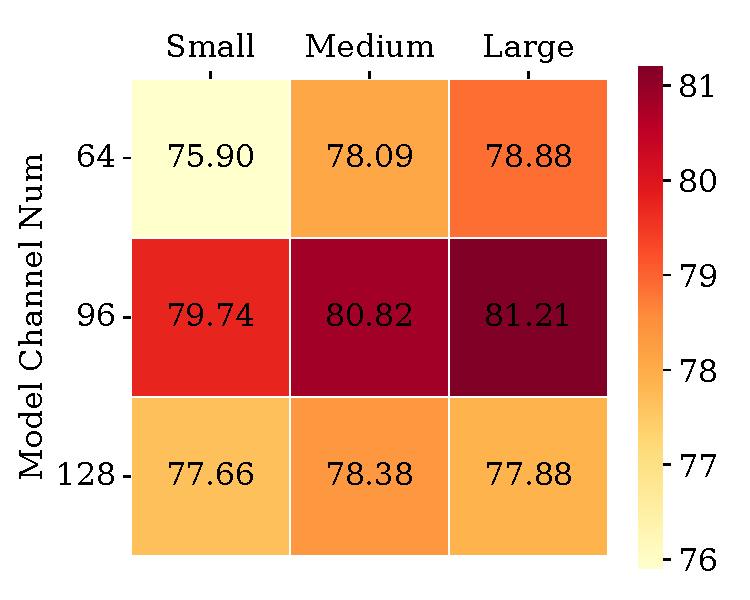
\includegraphics[width=\textwidth]{figure9.pdf}  % 左边图片文件名
        \caption{DSC Score Heatmap}
    \end{subfigure}
    \hfill
    \begin{subfigure}[b]{0.49\textwidth}
        \centering
        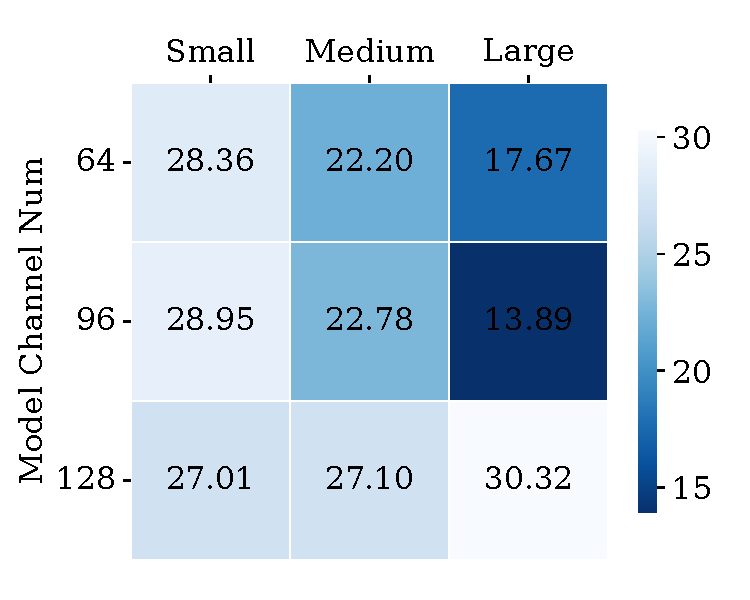
\includegraphics[width=\textwidth]{figure10.pdf}  % 右边图片文件名
        \caption{HD95 Score Heatmap}
    \end{subfigure}
    
    \caption{DSC scores (left) and HD95 scores (right) for models of different sizes under various channel configurations on the Synapse dataset.}
    \label{fig9}
\end{figure}
    
\textbf{Effect of Input Image Size:}
% 介绍输入图像大小的消融实验
To evaluate the impact of input image resolution on segmentation performance, we conducted experiments on the Synapse dataset using the DLKUNet-L model.
Specifically, we tested two input sizes: \(224\times 224\), \(512\times 512\) and recorded the DSC score for each resolution.

% 介绍消融实验的结果
The results showed in Table \ref{tab4} that increasing the input resolution led to a slight overall improvement in DSC, with a gain of 0.3\%.
Notably, the score for certain organs like the Aorta improved by 4.42\%, while others, such as the Stomach, experienced a decrease of approximately 10\%.
Additionally, increasing the input image size significantly raised the computational cost, with the floating point operations (FLOPs) increasing from \(29.64G\) to \(154.86G\).
Therefore, the input size is set \(224\times 224\) can provide a favorable balance between segmentation accuracy and computational resource consumption.

\begin{table}[h]
    \centering
    \caption{The impact of input datasets of different resolutions on DLKUNet-L and segmentation results in DSC score}
    \label{tab4}
    \begin{tabular*}{\textwidth}{@{\extracolsep{\fill}}lccccccccc}
        \toprule
        \textbf{Size} & \textbf{DSC} & \textbf{Aor} & \textbf{Gal} & \textbf{Kid(L)} & \textbf{Kid(R)} & \textbf{Liv} & \textbf{Pan} & \textbf{Spl} & \textbf{Sto} \\
        \midrule
        \(224\times 224\) & 81.21 & 87.39 & 67.40 & 87.64 & 83.47 & 92.41 & 63.44 & 90.99 & 76.92 \\
        \(512\times 512\) & \textbf{81.47} & \textbf{91.08} & \textbf{70.07} & 87.16 & 84.30 & \textbf{94.48} & \textbf{65.39} & 90.59 & 68.68 \\
        \bottomrule
    \end{tabular*}
\end{table}

\textbf{Effect of Kernel Size:}
% 介绍卷积核大小的消融实验
To investigate the effect of different kernel sizes on both the convolution part and the attention part, we designed several variations and tested them on the Synapse with an input size of \(224\times 224\).
Specifically, we experimented with four configurations listed in the Table \ref{tab5}.

\begin{table}[h]
    \centering
    \caption{Impact of different convolutional kernel configurations on the segmentation results using DLKUNet-L}
    \label{tab5}
    \begin{tabular*}{\textwidth}{@{\extracolsep{\fill}}lccc}
        \toprule
        \textbf{Models} & \textbf{Depthwise Kernel Size} & \textbf{Large Kernel Size} & \textbf{DSC} \\
        \midrule
        DLKUNet-L     & 3 $\times$ 3     & 5 $\times$ 5, 7 $\times$ 7  & \textbf{81.21} \\
        DLKUNet-5DW   & 5 $\times$ 5     & 5 $\times$ 5, 7 $\times$ 7  & 80.61 \\
        DLKUNet-7DW   & 7 $\times$ 7     & 5 $\times$ 5, 7 $\times$ 7  & 80.62 \\
        DLKUNet-LKA1  & 3 $\times$ 3     & 3 $\times$ 3, 7 $\times$ 7  & 80.68 \\
        DLKUNet-LKA2  & 3 $\times$ 3     & 5 $\times$ 5, 5 $\times$ 5  & 79.25 \\
        \bottomrule
    \end{tabular*}
\end{table}

Where DLKUNet-5DW and DLKUNet-7DW model replaced the \(3\times 3\) kernels of depthwise convolution in the DLKUNet-L model with \(5\times 5\) and \(7\times 7\) kernels, respectively.
DLKUNet-LKA1 and DLKUNet-LKA2 replaced the depthwise separable convolution in the attention part with a \(3\times 3\) kernel and a dilated convolution kernel of size \(5\times 5\).
The experimental results indicated that depthwise separable convolutions with kernel sizes of \(3\times 3\) and \(5\times 5\) achieved the best DSC scores on the Synapse dataset, while dilated convolutions performed optimally with a kernel size of \(7\times 7\).

\section{Discussion}\label{sec6}
In this paper, we propose DLKUNet, which demonstrates satisfactory overall performance in the task of multi-organ abdominal segmentation.
However, as shown in Figure \ref{fig10}, the performance in Pancreas segmentation is suboptimal, with DSC scores below 65, indicating significant limitations in handling such a complex organ.
This difficulty may be attributed to the complex anatomical structure, irregular shape, and significant variability in the position of the Pancreas, making it challenging to accurately identify and segment in medical images.
Additionally, the low contrast between the Pancreas and surrounding tissues further complicates the segmentation process, revealing the limitations of current models when dealing with organs that are morphologically complex and have fuzzy boundaries.
To enhance segmentation performance for the pancreas, future research could incorporate more advanced data augmentation techniques,
such as random rotations, translations, and scaling, to improve model robustness.
Additionally, utilizing more annotated medical image datasets or adopting transfer learning strategies could further enhance segmentation accuracy.
These methods could help models better handle organ variability and irregularity, improving segmentation accuracy for challenging tasks.

\begin{figure}[h]
    \centering
    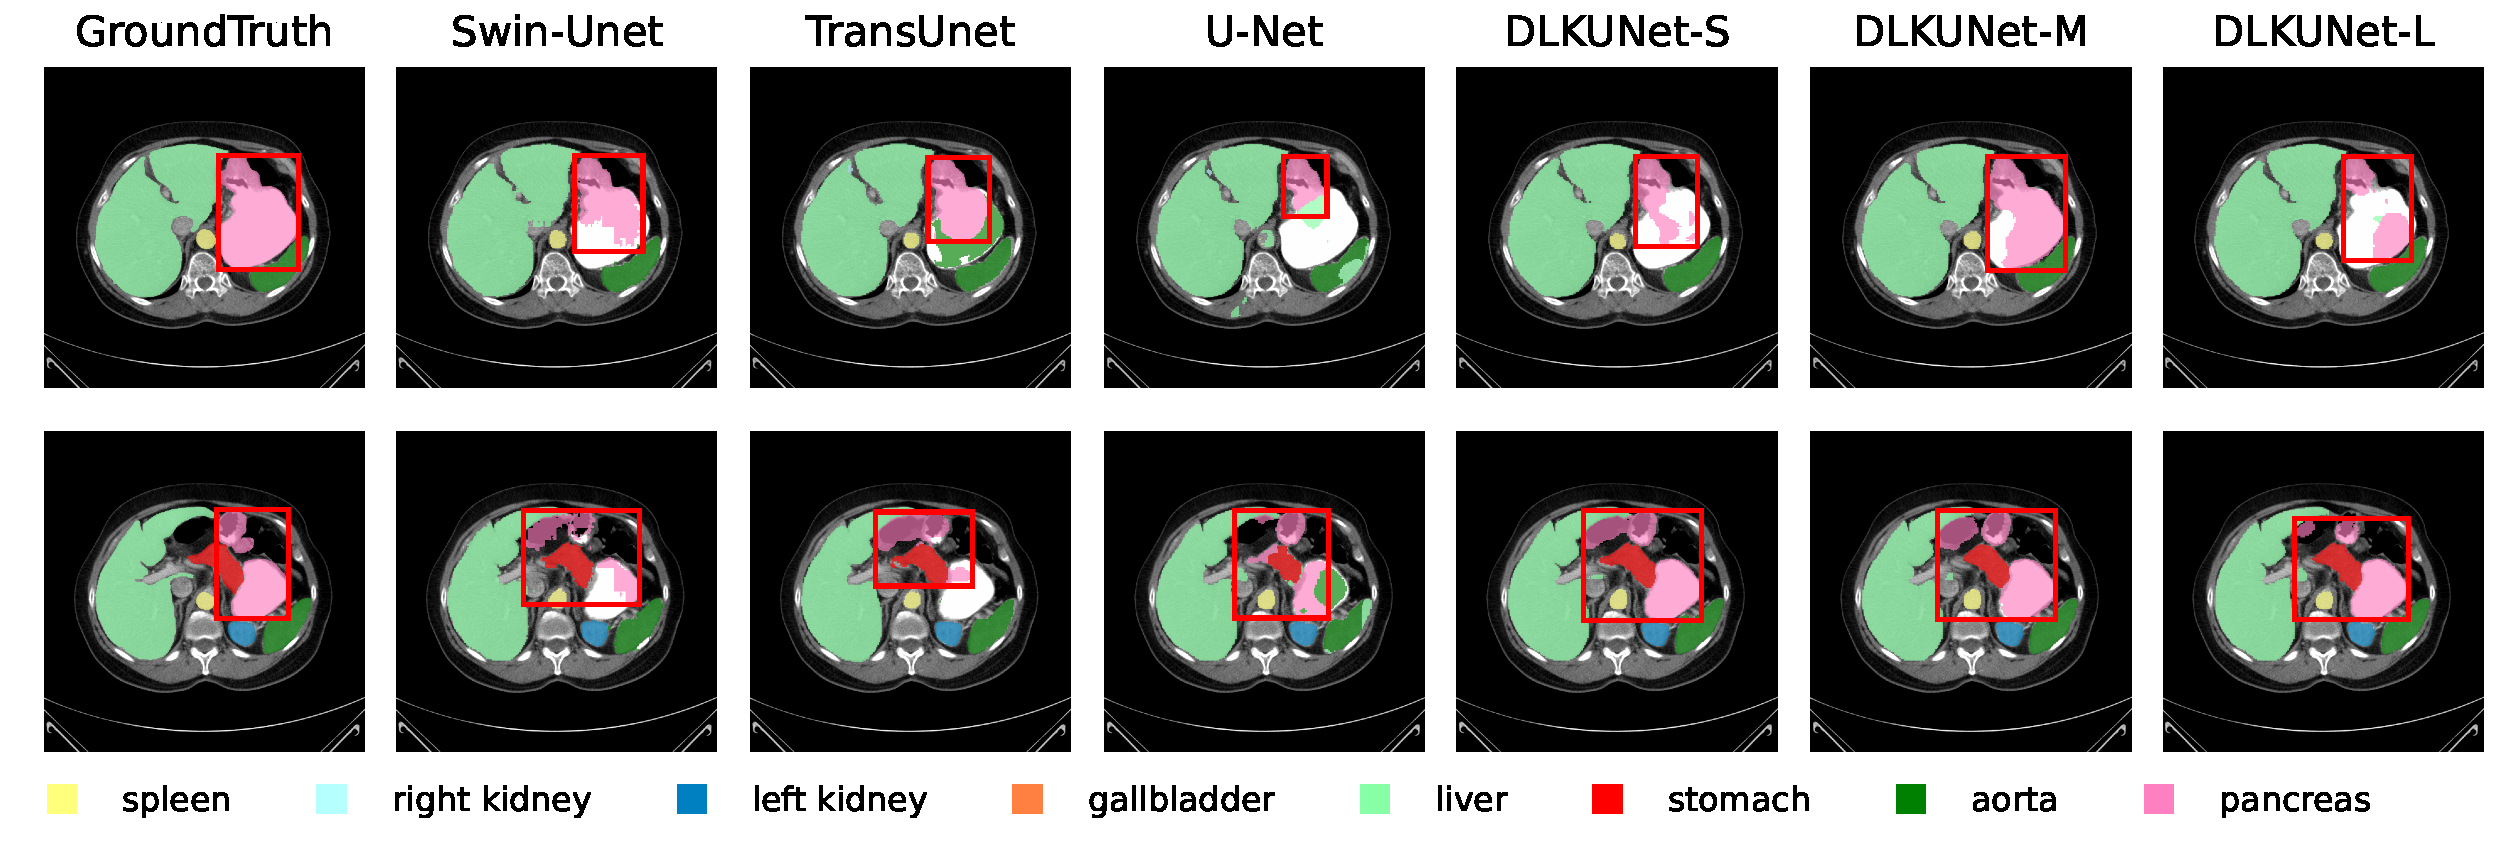
\includegraphics[width=\textwidth]{figure11.pdf}
    \caption{Segmentation Results for Pancreas Using Different Methods}\label{fig10}
\end{figure}

\section{Conclusion}\label{sec7}

In this study, we introduced an innovative method for medical image segmentation. 
The DLKUNet significantly improves segmentation accuracy through effective multi-scale feature extraction, enhancing the model's ability to capture key features across different scales.
We also designed several training optimization strategies, involving rational adjustments to loss function weights and dynamic learning rates, which accelerated model convergence and significantly improved training efficiency and accuracy.
We conducted extensive experiments on two public medical imaging datasets, Synapse and ACDC.
Results demonstrate that DLKUNet showed significant improvements in segmentation accuracy and parameter efficiency, validating the model's exceptional performance across different datasets and tasks.
In summary, DLKUNet shows outstanding performance in the field of medical image segmentation, with high parameter efficiency and computational performance, offering extensive support for future medical image analysis and clinical applications.

\bibliography{sn-bibliography}% common bib file
%% if required, the content of .bbl file can be included here once bbl is generated
%%\input sn-article.bbl

\end{document}